
% -------------------------------------------------------------------------------------------
\newpage\section{Input Equivalence Class Partitionings}\label{sec:iecpstart}

\subsection{Strategy Overview}\label{sec:strategyoverview}
In this section we summarise the main results of the novel equivalence class partitioning method, whose theory has been described in~\cite{peleska2013ictss}, before its application is illustrated in Section~\ref{sec:csmiecp}, using the CSM as an example.


In the exposition below, variable symbols $x,m,y$ are used with the convention that $x\in I, m\in M, y \in O$, and the symbols can be enumerated as  $I = \{ x_1,\dots,x_k\}$, $M = \{m_1,\dots, m_p\}$, $O = \{y_1,\dots,y_q\}$. We use   notation
$\vec x = (x_1,\dots,x_k), s(\vec x) = (s(x_1),\dots,s(x_k))$, $D_I = D_{x_1}\times\dots\times D_{x_k}$ denotes the cartesian product of the input variable domains. Tuples $\vec m, \vec y$ and $D_M$ and $D_O$ are defined over model variables and outputs in an analogous way. By $s\oplus\{\vec x \mapsto \vec c\}, \ \vec c \in D_I$ we denote the state $s'$ which coincides with $s$ on all variables from $M\cup O$, but returns values $s'(x_i) = c_i,\ i = 1,\dots,k$ for the input symbols. 

% ----------------------------------------------------------------
\subsubsection{I/O-Equivalence}\label{sec:ioequiv}

Applying a trace $\iota = \vec c_1\dots\vec c_n$ 
of input vectors $\vec c_i\in D_I$ to a STS $(S,s_0,R)$  residing in some quiescent state
$s\in S$, this stimulates a sequence of state transitions with associated  output changes  
as triggered by the inputs. Restricting this   sequence to quiescent states, this results in
a trace of states
$\tau = s_1.s_2\dots s_n$ such that $s_i(\vec x) = \vec c_i, i = 1,\dots,n$, and
$s_i(\vec y)$ is the last STS output resulting from application of $\vec c_1\dots\vec c_i$ 
to state $s$. This trace $\tau$ is generally denoted by $s/\iota$. The restriction of $s/\iota$ to output variables is denoted by $(s/\iota)|_O$.
Since transient states have unique quiescent post-states, the restriction to quiescent states does not result in a loss of information, if the input trace $\iota$ is known: the omitted transient states are some elements of $s\oplus\{\vec x \mapsto \vec c_1\},\dots,
s_{n-1}\oplus\{\vec x \mapsto \vec c_n\}$, and these states satisfy $R(s\oplus\{\vec x \mapsto \vec c_1\},s_1),\dots,R(s_{n-1}\oplus\{\vec x \mapsto \vec c_n\},s_n)$.

Two states $s, s'$ are {\it I/O-equivalent}, written $s\sim s'$, 
if every non-empty input trace $\iota$, when applied to $s$ and $s'$, results in the same outputs, that is,  
$(s/\iota)|_O = (s'/\iota)|_O$. Two STS ${\cal S}, {\cal S}'$ are I/O-equivalent, if their initial states 
are I/O-equivalent.
Note that for technical reasons, $s\sim s'$ still admits that $s|_O \neq s'|_O$.   

% ----------------------------------------------------------------
\subsubsection{Input Equivalence Class Partitions}\label{sec:iecp}

Since I/O-equivalence is an equivalence relation, we can factorise STS state spaces by $\sim$,
and the resulting equivalence classes $A \in S/_\sim$ have the property that all $s,s'\in A$ yield the same output traces $(s/\iota)|_O = (s'/\iota)|_O$  for arbitrary non-empty input traces $\iota$. For systems like the CSM, the number of classes $A$ is finite, so we can enumerate $S/_\sim = \{A_1,\dots,A_r\}$. Applying an arbitrary input vector $\vec c\in D_I$ to any state $s\in A_i$ will always lead to a quiescent target state -- denoted by $(s\trl \vec c)$  --
in the same target class $A_j$. 
%
%Index $j$ only depends on $(i,\vec c)$,   
%since for $s,s'\in A_i$ all corresponding states $s_i,s_i'$
%in $s/\iota = s_1.s_2\dots, s'/\iota= s_1'.s_2'\dots$ are I/O-equivalent. 
%
Index $j$ only depends on $(i,\vec{c})$, since for $s, s'\in A_i$ all corresponding
states $s_k, s_k'$ in $s/\iota=s_1.s_2\ldots .s_n, s'/\iota=s_1'.s_2'\ldots .s_n'$ are
I/O-equivalent for any $\iota=\vec{c}_1\ldots \vec{c}_n$, $k=1\ldots n$.


Therefore 
$(s\trl \vec c)\in A_j$ if and only if $(s'\trl \vec c)\in A_j$.
One class $A_j$, however, may contain elements $s \sim s'$ with different outputs, since I/O-equivalence only states that all future outputs will be identical, when applying the same non-empty input trace to $s,s'$. Since $D_O = \{ \vec d_1,\dots,\vec d_{|D_O|} \}$ is finite, we can associate
the value index $h\in \{1,\dots,|D_O|\}$ with the target class $A_j$, 
if $(s\trl \vec c)|_O = \vec d_h$. Again, $h$ only depends on $(i,\vec c)$, but not on the choice of $s\in A_i$.

Applying $\vec c$ to elements from all classes $A_1,\dots,A_r$, results in   (not necessarily distinct) index pairs $j(\vec c,i),h(\vec c,i),\ i= 1,\dots,r$.
This induces a factorisation of the input domain $D_I$:   
define $X(\vec c) \subseteq D_I$ as the maximal set containing $\vec c$, such that 
$j(\vec c',i) = j(\vec c,i) \wedge h(\vec c',i) = h(\vec c,i),\ i= 1,\dots,r,$ 
holds for   all $\vec c'\in X(\vec c)$. 

Then the {\it Input Equivalence Class Partitioning (IECP)}
${\cal I} = \{X(\vec c)~|~\vec c\in D_I\}$ has the following properties: (1) The elements of ${\cal I}$
are pairwise disjoint, (2) The union of all $X\in {\cal I}$ equals $D_I$, (3) ${\cal I}$ is finite,
and (4) for all $s\in A_i$, $\vec c\in X$, target states $(s\trl\vec c)$ are contained in the same target class $A_{j(i,\vec c)}$ and have the same output value $d_{h(i,\vec c)}$. Furthermore, each pair of input traces $\iota = \vec c_1\dots\vec c_n$, $\iota'= \vec c_1'\dots\vec c_n'$, when applied to the same state $s$, lead to the same output traces $(s/\iota)|_O = (s/\iota')|_O$, if
$\vec c_i' \in X(\vec c_i)$ for each $i=1,\dots,n$.  

A given IECP ${\cal I}$ can be {\it refined} by selecting input sets 
${\cal I}_2 = \{ X_1,X_2,\dots\}$ such that
${\cal I}_2$  also fulfils the above properties (1), (2), (3), and such that every $X_i$ is a subset of  
 some $X\in {\cal I}$. If these conditions hold, ${\cal I}_2$ inherits property (4). Refinement is obviously reflexive, transitive and anti-symmetric.

% ----------------------------------------------------------------
\subsubsection{Fault Model}\label{sec:faultmodel}

As reference models we use the STS representations ${\cal S}$ of models elaborated in concrete formalisms -- like the CSM model presented in this paper -- such that the expected behaviour of the SUT is specified by ${\cal S}$ up to I/O-equivalence. We use  I/O-equivalence as conformance relation.
The fault domain ${\cal D}$ specifies the set of potential systems under test, whose   true behaviour can be represented by an STS  ${\cal S}'\in {\cal D}$. For the equivalence class testing strategy, the
 fault domain depends on the reference model ${\cal S}$  and two additional parameters $m\in \N$ and
a refinement ${\cal I}_2$ of ${\cal I}$, the IECP associated with ${\cal S}$.  ${\cal D}({\cal S},m,{\cal I}_2)$ contains all ${\cal S}'$ satisfying 
\begin{enumerate}
\item The states of ${\cal S}'$ are defined over the same variable space $V = I\cup M \cup O$ as 
defined for the model ${\cal S}$.

\item Initial state $s_0'$ of ${\cal S}'$ coincides with initial state 
$s_0$ of ${\cal S}$ on $I\cup O$. 

\item ${\cal S}'$ generates only finitely many different output values and internal state values.

\item The number of I/O-equivalence classes of ${\cal S}'$ is less or equal $m$.

 

\item  Let ${\cal I}'$ be the IECP of  ${\cal S}'$ as defined above. Then  
$$
\forall X\in {\cal I}, X'\in {\cal I}': \big(X\cap X'\neq\varnothing \Rightarrow
\exists X_2\in {\cal I}_2: X_2 \subseteq X\cap X'\big)
$$

\item ${\cal S}'$ has a well-defined reset operation allowing to re-start the system, in order to perform another test from its initial state.

\end{enumerate}

Requirement~2 is well-founded, since initial states correspond to the system's switched-off state.
Therefore we can assume that the implementation produces the
same outputs as the reference model as long as it is switched off -- 
otherwise we would not start testing, because ${\cal S}$ and ${\cal S}'$ 
differed already in the off-state.

The fault domain ${\cal D}({\cal S},m,{\cal I}_2)$   is obviously 
increased by increasing $m\in \N$, and/or further refining ${\cal I}_2$:
$$
m' \ge m \wedge {\cal I}_3\ \text{refines}\ {\cal I}_2 \Rightarrow
 {\cal D}({\cal S},m,{\cal I}_2)\subseteq {\cal D}({\cal S},m',{\cal I}_3)
$$


% ----------------------------------------------------------------
\subsubsection{Complete Test Strategy}\label{sec:competestrat}

The main result of the paper~\cite{peleska2013ictss} states that, given reference model ${\cal S}$ and fixing $(m,{\cal I}_2)$, it is possible to generate a finite  test suite from ${\cal S}$, such that 
 (a) this suite accepts every member of  ${\cal D}({\cal S},m,{\cal I}_2)$ which is I/O-equivalent to ${\cal S}$, and (b) at least one test of this suite fails for every non-conforming member of
${\cal D}({\cal S},m,{\cal I}_2)$ 
which violates the I/O-equivalence condition. Test suites satisfying  (a) 
are called {\it sound}, and those satisfying (b) are called {\it exhaustive}. Soundness and exhaustiveness together  is called {\it complete}. The test suite is generated as follows.
\begin{enumerate}
\item Select one representative input vector $\vec c(X)$ from each   $X\in {\cal I}_2$.
\item Abstract ${\cal S}$ to a finite deterministic state machine ${\cal M}$ with I/O-equivalence classes $A_1,\dots,A_r$ as states, input alphabet $\{\vec c(X)~|~X\in {\cal I}_2\}$ and output alphabet 
$D_O$ (recall that $D_O$ is finite). This DFSM is well-defined due to the properties of the $A\in S/_\sim$ and the $X\in {\cal I}_2$.  
\item Since ${\cal M}$ is a DFSM, the well known W-Method~\cite{vasilevskii1973,chow:wmethod} 
% or the further optimised Wp-method~\cite{fujiwara:wpmethod} 
can be used to create a test suite that is complete with respect to reference model ${\cal M}$, conformance relation DFSM-equivalence, and the set of all DFSM over the same input/output alphabets as fault domain, whose
numbers of states do not exceed $m$.
\item A STS ${\cal S}'$ is I/O-equivalent to ${\cal S}$ if and only if its DFSM ${\cal M}'$ passes these tests, so that ${\cal M}'$ is DFSM-equivalent to ${\cal M}$. 
\end{enumerate}






% ====================================================================================
\subsection[Practical Construction of Input Equivalence Classes and Associated Partitionings]{Practical Construction of Input Equivalence Classes and\\Associated Partitionings}\label{sec:csmiecp}


%------------------------------------------------------------------------------------------ 

The set-theoretic introduction of IECP in Section~\ref{sec:strategyoverview} 
have a propositional counterpart in the formulas introduced above in the context of the transition relation. This propositional view is needed for  being able to calculate concrete representatives of IECP with the help of an constraint solver.

% --------------------------------------------------------------------------
\subsubsection{CSM I/O-Equivalence Classes}\label{sec:csmioeq}
  
Reviewing the CSM transition relation shown in Formulas~(\ref{eq:rcsm} --- \ref{eq:phik4}),
the identification of quiescent I/O equivalence classes is straightforward: they are identical to or unions of the quiescent state sets
\begin{equation}
\label{eq:aicsm}
A_i = \{ s\in S~|~s(\varphi_i)  \},\ \ i = 0,\dots,4,\ \ \text{$\varphi_i$ as defined in formulas~(\ref{eq:phi0} --- \ref{eq:phi4})}
\end{equation}
To see this, let us first show that each $A_i$ only contains I/O-equivalent states, so that it is a subset of an I/O equivalence class.  This follows directly from the following observations about the CSM transition relation.
\begin{enumerate}
\item If one quiescent state $s$ from $A_i$ can transit to a transient state $s'$ in set
$$
B_j = \{s~|~s(\varphi_{k_0+j})\},\ \ j = 0,\dots,4
$$
by an input change $s' = s\oplus\{(\vest,\vmax,\areb) \mapsto (c_1,c_2,c_3)\}$
then {\it all} elements of $A_i$ can transit to $B_j$ with the same input change $(\vest,\vmax,\areb) \mapsto (c_1,c_2,c_3)$.

\item All elements of $B_j$ have post-states in the same quiescent state set $A_j$, uniquely determined by the fact that these post-states   must satisfy $\xi_j$, that is, must have the same outputs and the same internal state.
\end{enumerate}

From the calculations performed for the CSM transition relation (Section~\ref{sec:transientinputcond}) we know that $\varphi_{0,i}^I \equiv \varphi_{1,i}^I, i = 2,3,4$,  
$\varphi_0\equiv \varphi_{1,0}^I$, and $\varphi_{0,1}^I \equiv \varphi_1$. This implies that $A_0$ and $A_1$ are I/O-equivalent. Similarly, it can be deduced that $A_0\cup A_1,A_2, A_3, A_4$ are 
pairwise distinguishable with respect to I/O-equivalence, so these four sets are the I/O-equivalence classes of the CSM's STS.


% --------------------------------------------------------------------------
\subsubsection{CSM Input Equivalence Class Partitions}\label{sec:csmiecpxxx}

As described in Section~\ref{sec:iecp}, we need the refined quiescent state sets
for the identification of IECP,  resulting from I/O-equivalence classes further partitioned in a way that the states of each resulting set have identical output valuations. These are exactly the sets $A_0,\dots,A_4$ from equation~(\ref{eq:aicsm}), since the
formulas $\varphi_i$ defining the $A_i$ specify the constant output values.

The input equivalence class partitions introduced in  Section~\ref{sec:iecp} can be expressed in a propositional way by specifying
\begin{equation}
{\cal I} = \{ X=\{\vec c\in D_i~|~\bigwedge_{i=0}^4 \varphi_{q,j_i}^I[\vec c/(\vest,\vmax,\areb)]\}~|~j_i\in \{0,\dots,4\}
\wedge X\neq \varnothing   \}
\end{equation}
In this definition the   $\varphi_{q,j_i}^I$ are defined as in Equation~(\ref{eq:phiIa} --- \ref{eq:phiIz}), for $q \neq j_i$, and $\varphi_{q,q}^I \equiv \varphi_q^I$, with $\varphi_q^I$ defined in 
Equation~(\ref{eq:phiI0} --- \ref{eq:phiI4}). 
  
  
  
For the CSM, the feasible non-equivalent propositions $\Phi_k \equiv \bigwedge_{i=0}^4 \varphi_{q,j_i}^I$ are
\begin{eqnarray*}
\Phi_1 & \equiv & \varphi_{0,0}^I \wedge \varphi_{1,0}^I \wedge \varphi_{2,0}^I \wedge \varphi_{3,0}^I \wedge \varphi_{4,4}^I
\\ & \equiv & \varphi_{0,0}^I \wedge \varphi_{4,4}^I
\\ & \equiv & 0 < \vest \le \vmax \wedge \areb = 0
\\
\Phi_2 & \equiv & \varphi_{0,0}^I \wedge \varphi_{1,0}^I \wedge \varphi_{2,0}^I \wedge \varphi_{3,0}^I \wedge \varphi_{4,0}^I
\\ & \equiv & \varphi_{4,0}^I
\\ & \equiv & \vest = 0 \vee (\vest \le \vmax \wedge \areb = 1)
\\
\Phi_3 & \equiv & \varphi_{0,1}^I \wedge \varphi_{1,1}^I \wedge  \varphi_{2,2}^I \wedge \varphi_{3,3}^I \wedge \varphi_{4,4}^I 
\\ & \equiv & \varphi_{0,1}^I \wedge \varphi_{4,4}^I
\\ & \equiv & (\vmax \le 110 \wedge   \vmax <  \vest \le \vmax +4) \vee {}
\\ & & (110<\vmax  \le 140  \wedge \vmax < \vest \le \frac{31}{30}\vmax +\frac{1}{3} )
\vee {}
\\ & & (140<\vmax \wedge  \vmax < \vest \le \vmax +5) 
\\
\Phi_4 & \equiv & \varphi_{0,2}^I \wedge \varphi_{1,2}^I \wedge \varphi_{2,2}^I \wedge  \varphi_{3,3}^I \wedge \varphi_{4,4}^I 
\\ & \equiv & \varphi_{0,2}^I \wedge \varphi_{4,4}^I
\\ & \equiv & (\vmax \le 110 \wedge \vmax +4 < \vest \le \vmax + 5.5 )
\vee {}
\\ & &  (110 <\vmax  \le 140 \wedge \frac{31}{30}\vmax +\frac{1}{3} < \vest \le\frac{209}{200}\vmax +\frac{55}{100}) \vee {}
\\ & & (140 < \vmax \le 210 \wedge \vmax +5 < \vest \le\frac{209}{200}\vmax +\frac{55}{100}) \vee {}
\\ & &  (210 < \vmax  \wedge  \vmax +5 < \vest \le\vmax + 10)
\end{eqnarray*}

\begin{eqnarray*}
\Phi_5 & \equiv & \varphi_{0,3}^I \wedge \varphi_{1,3}^I \wedge  \varphi_{2,3}^I \wedge \varphi_{3,3}^I \wedge \varphi_{4,4}^I 
\\ & \equiv & \varphi_{0,3}^I 
\\ & \equiv & (\vmax \le 110 \wedge \vmax + 5.5 < \vest \le  \vmax + 7.5) \vee {}
\\ & & (110<\vmax \le 210 \wedge \frac{209}{200}\vmax +\frac{55}{100}< \vest \le  \frac{43}{40}\vmax -\frac{3}{4}) \vee {}
\\ & & (210<\vmax   \wedge \vmax +10 < \vest \le  \vmax +15)
\\
\Phi_6 & \equiv & \varphi_{0,4}^I \wedge \varphi_{1,4}^I \wedge \varphi_{2,4}^I \wedge \varphi_{3,4}^I \wedge \varphi_{4,4}^I \wedge
\\ &\equiv & \varphi_{0,4}^I
\\ &\equiv & (\vmax \le 110 \wedge \vmax + 7.5 < \vest ) \vee {}
\\ & & (110<\vmax \le 210 \wedge  \frac{43}{40}\vmax -\frac{3}{4}< \vest ) \vee {}
\\ & & (210<\vmax   \wedge \vmax +15 < \vest )
\end{eqnarray*}


With these definitions, the IECP is given by
\begin{eqnarray}
{\cal I} & = & \{ X_1,\dots,X_6  \}
\\
X_i & = & \{\vec c\in D_I~|~\Phi_i[\vec c/(\vest,\vmax,\areb)]\},\ \ \ i = 1,\dots,6
\end{eqnarray}
The properties of this IECP will be discussed in the subsequent sections, and we will also discuss the necessity for IECP refinements.
 
% ----------------------------------------------------------------------
\subsection{Inter-Class Transitions}

With the IECP at hand, the state transition system representing the behavioural semantics of the SysML state machine can be abstracted to a deterministic finite  state machine (DFSM): Each $X_i$ introduced above, or a representative value of each $X_i$, represents an event of the state machine, and the classes $A_i, B_i$ are the  DFSM states. The  DFSM transition table is specified in Table~\ref{tab:tr}.


\begin{table}[htdp]
\caption{DFSM Transition Table.}
\begin{center}
\begin{tabular}{|c||c||c||c||c|c|}
\hline\hline
{\bf Source}& {\bf Input} & {\bf via} & {\bf Target}&$\mathbf{\dmicmd}$&$\mathbf{\ticmd}$ \\\hline\hline
$A_0$&$X_1\cup X_2$& --- & $A_0$&0&0 \\
$A_0$&$X_3$& $B_1$ &$A_1$&2&0\\
$A_0$&$X_4$& $B_2$  &$A_2$&3&0\\
$A_0$&$X_5$& $B_3$  &$A_3$&4&2-$\sbz$ \\
$A_0$&$X_6$& $B_4$ &$A_4$&4&2 \\

\hline
$A_1$&$X_1\cup X_2$& $B_0$ &$A_0$&0&0\\
$A_1$&$X_3$& --- & $A_1$&2&0 \\
$A_1$&$X_4$& $B_2$ & $A_2$&3&0 \\
$A_1$&$X_5$& $B_3$ & $A_3$&4&2-$\sbz$ \\
$A_1$&$X_6$& $B_4$ &$A_4$&4&2\\
\hline
$A_2$&$X_1\cup X_2$& $B_0$ &$A_0$&0&0 \\
$A_2$&$X_3\cup X_4$& --- &$A_2$&3&0 \\
$A_2$&$X_5$& $B_3$ & $A_3$&4&2-$\sbz$\\
$A_2$&$X_6$& $B_4$ &$A_4$&4&2 \\
\hline
$A_3$&$X_1\cup X_2$& $B_0$ &$A_0$&0&0\\
$A_3$&$X_3\cup X_4\cup X_5$& --- &$A_3$&4&2-$\sbz$ \\
$A_3$&$X_6$& $B_4$ &$A_4$&4&2 \\
\hline
$A_4$&$X_2$& $B_0$ &$A_0$&0&0\\
$A_4$&$\bigcup_{i\in\{1,3,4,5,6\}}X_i$& --- &$A_4$&4&2 
\\\hline\hline
\end{tabular}
%\normalsize
\end{center}
\label{tab:tr}
\end{table}

For concrete tests we select representatives of each IEC, such as the ones specified in Table~\ref{tab:inputalphabet}. The set of these representatives is called the {\it input alphabet} ${\cal A}_I$.


\begin{table}[htdp]
\caption{Input Alphabet ${\cal A}_I$.}
\begin{center}
\begin{tabular}{|c||c|c|c||c|}
\hline\hline
$\vec c_i$&$\vest$&$\vmax$&$\areb$&$X_i$ \\\hline\hline
$\vec c_1$&60&90&0&$X_1$ \\
$\vec c_2$&60&90&1&$ X_2$ \\
$\vec c_3$&152&150&0&$X_3$\\
$\vec c_4$&125&120&1&$X_4$\\
$\vec c_5$&66&60&0&$X_5$ \\
$\vec c_6$&260&230&0&$X_6$
\\\hline\hline
\end{tabular}
%\normalsize
\end{center}
\label{tab:inputalphabet}
\end{table}


 



% =============================================================================
\section{CSM Fault Model}\label{sec:testhypo}

The fault model introduced in Section~\ref{sec:faultmodel} is instantiated for the CSM as follows.
\begin{itemize}
\item The reference model for the CSM is the STS ${\cal S}$ defined in Section~\ref{sec:transrel}.
\item We use  I/O-equivalence as conformance relation, as introduced in Section~\ref{sec:ioequiv}.
\item We will consider several fault domains, starting with
$$
{\cal D}({\cal S},m=6,{\cal I}_2 = {\cal I})
$$
where $m$ denotes the upper bound of I/O-equivalence classes occurring in (conforming or non-conforming) implementations of ${\cal S}$, and ${\cal I}$ is the IECP constructed in Section~\ref{sec:csmiecpxxx}.
\end{itemize}

The assurance gained from performing a completed test suite with respect to fault domain  ${\cal D}({\cal S},m=6,{\cal I}_2 = {\cal I})$ will be discussed below in Section~\ref{sec:test-strength}, and meaningful refinements of  ${\cal D}({\cal S},m=6,{\cal I}_2 = {\cal I})$ are introduced in Section~\ref{sec:refineheuristics}.



% ===============================================================================
\section{Complete Test Suites for the CSM}\label{sec:completesuites}


\subsection{Test Suite Construction -- Overview}
Applying the recipe for complete test strategies specified in Section~\ref{sec:competestrat}, such a test suite can be constructed for the CSM as follows.
\begin{enumerate}
\item The input alphabet ${\cal A}_I$ consists of the vectors $\vec c_i$ selected from each of the IEC $\{X_1,\dots,X_6\}$, as specified in Table~\ref{tab:inputalphabet}.

\item For each of the two configurations ``with service brake ($\sbz = 1$)'', and ``without service brake ($\sbz = 0$)'' a DFSM is constructed with state space $\{q_0 = A_0\cup A_1,q_2 = A_2,q_3 = A_3,q_4 = A_4\}$ and initial state
$A_0\cup A_1$; these I/O-equivalence classes have been identified above in 
Section~\ref{sec:csmioeq}. 
Each state machine operates on input alphabet ${\cal A}_I$ and output alphabet $D_O$, and their transition functions are specified by Table~\ref{tab:tr}.

The resulting DFSMs are  shown in Figure~\ref{fig:dfsmcsm}, with $\sbz \in \{0,1\}$ to be fixed according to the train configuration. In Table~\ref{tab:AandMinDFSM} the mapping of DFSM state names to I/O-equivalence classes is shown.

\item For each of the two DFSM a test suite is constructed according to the W-method, as described below.
\end{enumerate}

\begin{table}[htdp]
\caption{DFSM states and associated I/O-equivalence classes.}
\begin{center}
\footnotesize
\begin{tabular}{|c|c|c|}
\hline\hline
{\bf DFSM State} & {\bf DFSM State Name} & {\bf I/O-Equivalence Class}
\\\hline\hline
$q_0$ & {\sf Normal or Overspeed} & $A_0\cup A_1$ 
\\\hline
$q_2$ & {\sf Warning} & $A_2$ 
\\\hline
$q_3$ & {\sf Service Brake Intervention} & $A_3$ 
\\\hline
$q_4$ & {\sf Emergency Brake Intervention} & $A_4$ 
\\\hline\hline
\end{tabular}
\normalsize
\end{center}
\label{tab:AandMinDFSM}
\end{table}%

 \begin{figure}
 %%\hspace*{-40mm}
 \begin{center}
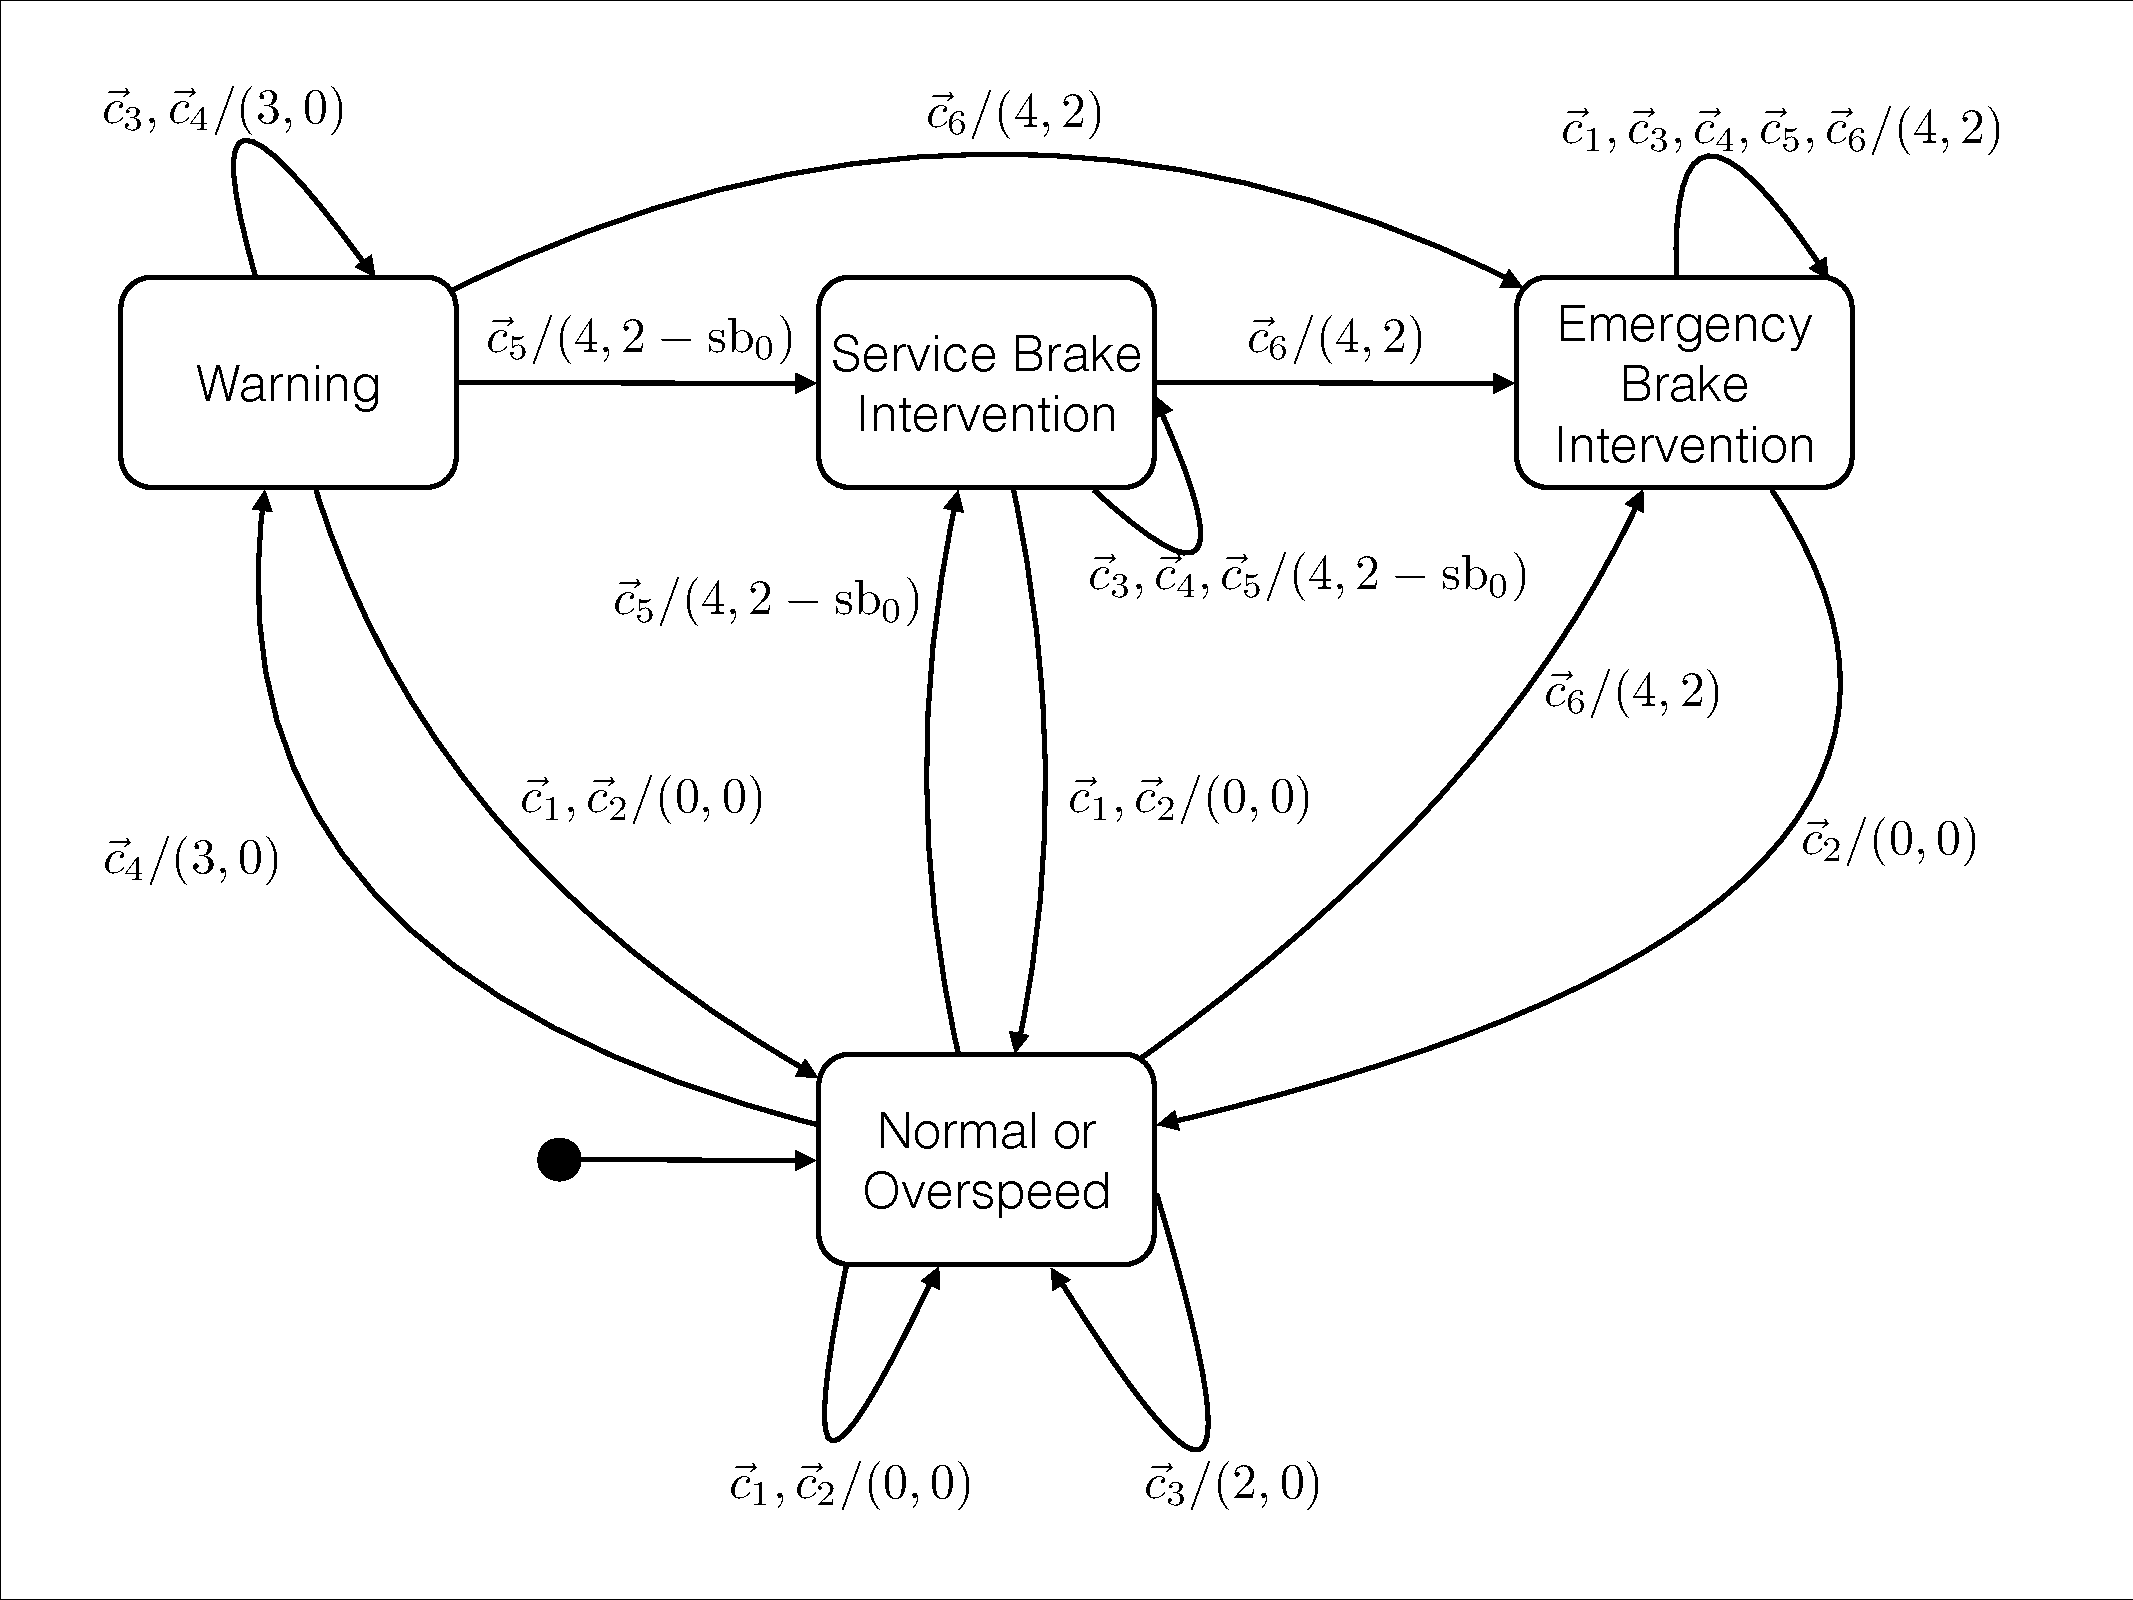
\includegraphics[width=0.8\textwidth]{dfsm0.pdf}
%%\vspace*{-35mm}

 \footnotesize
 \bigskip
 Output assignment actions $(\dmicmd,\ticmd) = (\alpha,\beta)$ are written as $(\alpha,\beta)$.
 \normalsize
\end{center}
\caption{DFSM abstractions of the CSM, with configuration cases $\sbz\in\{0,1\}$.}
 \label{fig:dfsmcsm}
 \end{figure}



% ----------------------------------------------------------------------------------
\subsection{Application of the W-Method}

For application of the W-Method on the given DFSMs, we need to identify two sets of input traces, the {\it state-transition cover $STC$} and the 
{\it characterisation set $W$}~\cite{chow:wmethod,vasilevskii1973}.

% ....................................................................................
\paragraph{State-transition cover.} $STC$ is constructed as a set of traces fulfilling
\begin{enumerate}
\item  The empty trace is a member of $STC$.
\item For any reachable state $q$ and any $\vec c\in {\cal A}_I $, there is an input trace 
$\iota\in STC$ such that 
\begin{itemize}
\item $q$ can be reached from the initial state of the DFSM by application of $\iota$, and
\item $\iota.\vec c\in STC$.
\end{itemize}
\end{enumerate}

For the DFSMs under consideration, a state-transition cover is given by 
$$
STC=\{\varepsilon, \vec c_i, \vec c_j.\vec c_i~|~i=1,\dots,6,\  j=4,\dots,6\}
$$

% ....................................................................................
\paragraph{Characterisation set.} $W$ is defined as a set of input traces distinguishing all DFSM states (recall that the DFSM under consideration are minimal) in the sense that for every pair
of DFSM states $q,q'$, there exists an input trace $\tau\in W$ such that $\tau$ applied to $q$
yields an output sequence which differs from the one resulting from application of $\tau$ in state
$q'$.
For the case where the service brake differs from the emergency brake ($\sbz = 1$), the single input
$$
W_{\sbz=1}=\{\vec c_3\}  
$$
distinguishes all states of $\text{DFSM}$, as can be directly seen in Figure~\ref{fig:dfsmcsm}. In the case where the emergency brake is used for service brake intervention ($\sbz = 0$), we need additional input $\vec c_1$ to distinguish DFSM states $q_3$ and $q_4$.
$$
W_{\sbz=0}=\{\vec c_1, \vec c_3\}  
$$

% ....................................................................................
\paragraph{Test suite according to W-Method.} With $STC$ and $W$ at hand, the W-Method asserts that the following test suite is complete for the fault domain of all DFSMs over the same input and output alphabets, whose state space has cardinality less or equal to $m$.
$$
{\cal W}(STS) = STC.({\cal A}_I)^{\max\{m,n\}-n}.W
$$
We use notation $({\cal A})^k$ to denote the subset of ${\cal A}^*$ containing all traces of length zero to $k$. ${\cal W}(STS)$ consists of all input traces starting with a (potentially empty) trace from the state-transition cover, continuing with a sequence of arbitrary inputs from the alphabet with length less or equal to $(\max\{m,n\}-n)$ (including the empty sequence), and ending with an input sequence contained in the transition cover.
$({\cal A})^0$ just contains the empty trace, so ${\cal W}(STS)$ is reduced to 
$STC.W$, if the fault domain of DFSM whose state space is less or equal to that of the reference DFSM is considered.

 
Assuming that the minimal DFSM associated with the SUT implements at most two additional states ($m-n\le 2$ implies $m\le 6$), the W-Method produces the following test suite for the the minimal DFSM:

\begin{eqnarray*}
STC.({\cal A}_I)^{2}.W_{\sbz=1}  & = & \{ \vec c_3\} \cup{}
\\ & & 
\{\vec c_i.\vec c_3~|~i=1,\dots,6\} \cup{}
\\ & &
\{\vec c_i.\vec c_j.\vec c_3~|~i,j=1,\dots,6\} \cup{}
\\ & &
\{\vec c_i.\vec c_j.\vec c_k.\vec c_3~|~i,j,k=1,\dots,6\} \cup{}
\\ & &
\{\vec c_j.\vec c_i.\vec c_3~|~i=1,\dots,6, \ \ j = 4,\dots,6 \} \cup{}
\\ & &
\{\vec c_j.\vec c_i.\vec c_k.\vec c_3~|~i,k=1,\dots,6, \ \ j = 4,\dots,6 \} \cup {}
\\ & & 
\{\vec c_j.\vec c_i.\vec c_k.\vec c_h.\vec c_3~|~h,i,k=1,\dots,6, \ \ j = 4,\dots,6 \}
\\ & & 
\\
STC.({\cal A}_I)^{2}.W_{\sbz=0}  & = & \{ \vec c_g~|~g=1,3 \}  \cup{}
\\ & & 
\{\vec c_i.\vec c_g~|~i=1,\dots,6,\ g=1,3\} \cup{}
\\ & &
\{\vec c_i.\vec c_j.\vec c_g~|~i,j=1,\dots,6,\ g=1,3\} \cup{}
\\ & &
\{\vec c_i.\vec c_j.\vec c_h.\vec c_g~|~h,i,j=1,\dots,6,\ g=1,3\} \cup{}
\\ & &
\{\vec c_j.\vec c_i.\vec c_g~|~i=1,\dots,6, \ \ j = 4,\dots,6,\ g=1,3 \} \cup{}
\\ & &
\{\vec c_j.\vec c_i.\vec c_k.\vec c_g~|~i,k=1,\dots,6, \ \ j = 4,\dots,6,\ g=1,3 \} \cup {}
\\ & &
\{\vec c_j.\vec c_i.\vec c_k.\vec c_h.\vec c_g~|~h,i,k=1,\dots,6, \ \ j = 4,\dots,6,\ g=1,3 \}
\end{eqnarray*}

Since $\iota$-equivalence implies $\tau$-equivalence when $\tau$ is a prefix of $\iota$, the test suite produced by the W-Method can be reduced to the following:
\begin{eqnarray*}
\text{TEST\_SUITE}_{\sbz=1} & = & 
\{\vec c_i.\vec c_j.\vec c_k.\vec c_3~|~i,j,k=1,\dots,6\} \cup{}
\\ & &
\{\vec c_j.\vec c_i.\vec c_k.\vec c_h.\vec c_3~|~h,i,k=1,\dots,6, \ \ j = 4,\dots,6 \}
\\ & & 
\\
\text{TEST\_SUITE}_{\sbz=0} & = & \{\vec c_i.\vec c_j.\vec c_h.\vec c_g~|~h,i,j=1,\dots,6,\ g=1,3\} \cup{}
\\ & &
\{\vec c_j.\vec c_i.\vec c_k.\vec c_h.\vec c_g~|~h,i,k=1,\dots,6, \ \ j = 4,\dots,6,\ g=1,3 \}
\end{eqnarray*}






 

 
% ==================================================================================
\section{Test Strength}
\label{sec:test-strength}
\subsection{Test Strength Assessment}

The notion of {\it test strength} refers to the capability of test suites to uncover   errors in an SUT. The IECP testing strategy considered here is associated with a well-defined test strength, specified by means of the fault model: all deviations of an SUT from I/O-equivalence to the reference model ${\cal S}$ will be detected, provided that the true behaviour of the SUT can be specified by means of an STS which is contained in the fault domain. Based on the fault domain, the discussion of test strength is ``transformed'' into the question  whether the size of the fault domain for which the test suite has been created is sufficient to contain all erroneous behaviours we can reasonably expect.
 
 
In the next three sections examples will be presented where the erroneous SUT behaviour can already by uncovered with IECP test suites based on the fault domain ${\cal D}({\cal S},m=6,{\cal I}_2={\cal I})$ specified in Section~\ref{sec:testhypo}.   
The first example (Section~\ref{sec:ex1}) addresses a type of erroneous behaviour that could not only be uncovered by the equivalence class testing strategy described in this report, but is also 
guaranteed to be detected by test suites achieving transition coverage of the SysML state machine model (see Section~\ref{sec:conventionaltests}). The second example (Section~\ref{sec:example2}) shows a type of failure that is {\it not guaranteed} to be uncovered by test cases from a simple model coverage strategy like transition or MC/DC coverage, because it introduces an additional basic state in the SUT's SysML state machine. Practical test execution documented in Section~\ref{sec:conventionaltests}, however, shows that  the failure is ``accidentally'' uncovered 
with the transition coverage strategy by the model-based testing tool used, due to suitable input values selected by the tool when trying to cover the required transitions.
The third example (Section~\ref{sec:example3}) exhibits an even harder failure type, which cannot be detected by any of the transition-based coverage strategies, as is documented by the test results
shown in Section~\ref{sec:conventionaltests}.  

In Section~\ref{sec:refineheuristics} we will discuss   fault models associated with 
larger fault domains, based on true refinements  of ${\cal I}$.




% ----------------------------------------------------------------------------------
\subsection{Example~1}\label{sec:ex1}

Suppose that the implementation acts like the SysML state machine depicted in 
Fig.~\ref{fig:transfail}: from basic state {\sf OVERSPEED} there is a transition failure in the SysML state machine which links to basic state {\sf EMER\_BRAKE} instead of {\sf NORMAL}, when guard condition $[\vest\le\vmax]$ evaluates to $\ist$. Note that the DFSM associated with $STS'$ now has one more state than the model's DFSMs, because {\sf OVERSPEED} and {\sf NORMAL} are no longer equivalent.

Assuming the case $\sbz=1$ and applying $\text{TEST\_SUITE}_{\sbz=1}$ introduced in Section~\ref{sec:completesuites}, this failure will be uncovered, for example, by test case
\footnotesize
\begin{eqnarray*}
\iota & = &\vec c_1. \vec c_3.\vec c_1.\vec c_3 
\\ & = & (\vest=60,\vmax=90,\areb=0).(152,150,0).(60,90,0).(152,150,0)
\end{eqnarray*}
\normalsize
On the model $STS$, this input will trigger output sequence
$$
(\dmicmd=0,\ticmd=0).(2,0).(0,0).(2,0)
$$
whereas output sequence
$$
(\dmicmd=0,\ticmd=0).(2,0).(4,2).(4,2)
$$
will be triggered by $\iota$, when applied to $STS'$ representing the SUT. 
 
 \begin{figure}
 \hspace*{-20mm}
%% \begin{center}
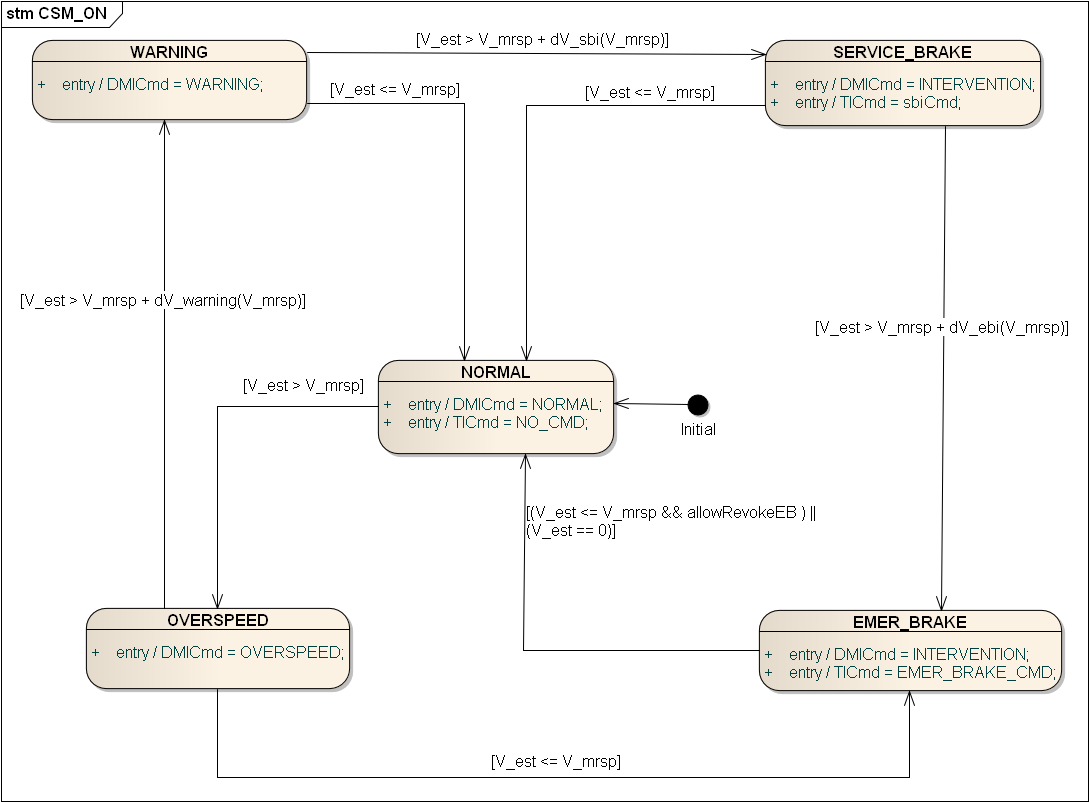
\includegraphics[width=1.3\textwidth]{CSM_ON_TRANSITION_FAILURE.png}
%%\vspace*{-35mm}
%%\end{center}
\caption{Faulty SUT -- Example~1.}
 \label{fig:transfail}
 \end{figure}


%-----------------------------------------------------------------------
\subsection{Example 2}\label{sec:example2}

Suppose that the implementation has an additional  control state $\text{NORMAL\_2}$, as depicted in Fig.~\ref{fig:addstatefail}. When the SUT is in the control state $\text{OVERSPEED}$ and inputs satisfy $\vest\le \vmax$, the SUT's state machine transits to the new basic state  
$\text{NORMAL\_2}$. For this control state, there is only one outgoing transition whose guard condition is $ \vest > \vmax + dV_{\text {ebi}}$, and target control state is $\text {EMER\_BRAKE}$.
As a consequence, the SUT fails to issue warnings and to trigger service brake intervention, after having entered $\text{NORMAL\_2}$; only the emergency brake intervention condition is handled correctly. The SUT failure remains hidden until a transition sequence from {\sf NORMAL} to {\sf OVERSPEED} and back to {\sf NORMAL} should be performed. Note that the introduction of this additional basic state in the SUT's SysML state machine leads to a DFSM abstraction that has {\it two} more states than the DFSM abstraction of the original model, because basic states {\sf NORMAL} and {\sf OVERSPEED} are no longer equivalent, and {\sf NORMAL\_2} is non-equivalent to any of the other states.


Assuming again the case $\sbz=1$ and applying $\text{TEST\_SUITE}_{\sbz=1}$ introduced in Section~\ref{sec:completesuites}, this failure will be uncovered, for example, by test case
\footnotesize
\begin{eqnarray*}
\iota & = & \vec c_3.\vec c_1.\vec c_4.\vec c_3 
\\ & = & (\vest=152,\vmax=150,\areb=0).(60,90,0).(125,120,1).(152,150,0)
\end{eqnarray*}
\normalsize
On the model $STS$, this input will trigger output sequence
$$
(\dmicmd=2,\ticmd=0).(0,0).(3,0).(3,0)
$$
whereas output sequence
$$
(\dmicmd=2,\ticmd=0).(0,0).(0,0).(0,0)
$$
will be triggered by $\iota$, when applied to $STS'$ representing the SUT. 

Observe that this SUT failure would not be uncovered by every ordinary transition coverage test strategy based on SysML state machine model. Transition coverage would be achieved, for example, by the four test cases
\begin{eqnarray*}
\text{TC\_TEST\_SUITE} & = & \{ \vec c_3.\vec c_1, \vec c_3.\vec c_4.\vec c_1,\vec c_4.\vec c_5.\vec c_1,\vec c_5.\vec c_6.\vec c_2  \}  
\end{eqnarray*}
which fail to uncover the violation of I/O-equivalence.

 



 
 \begin{figure}
 \hspace*{-20mm}
%% \begin{center}
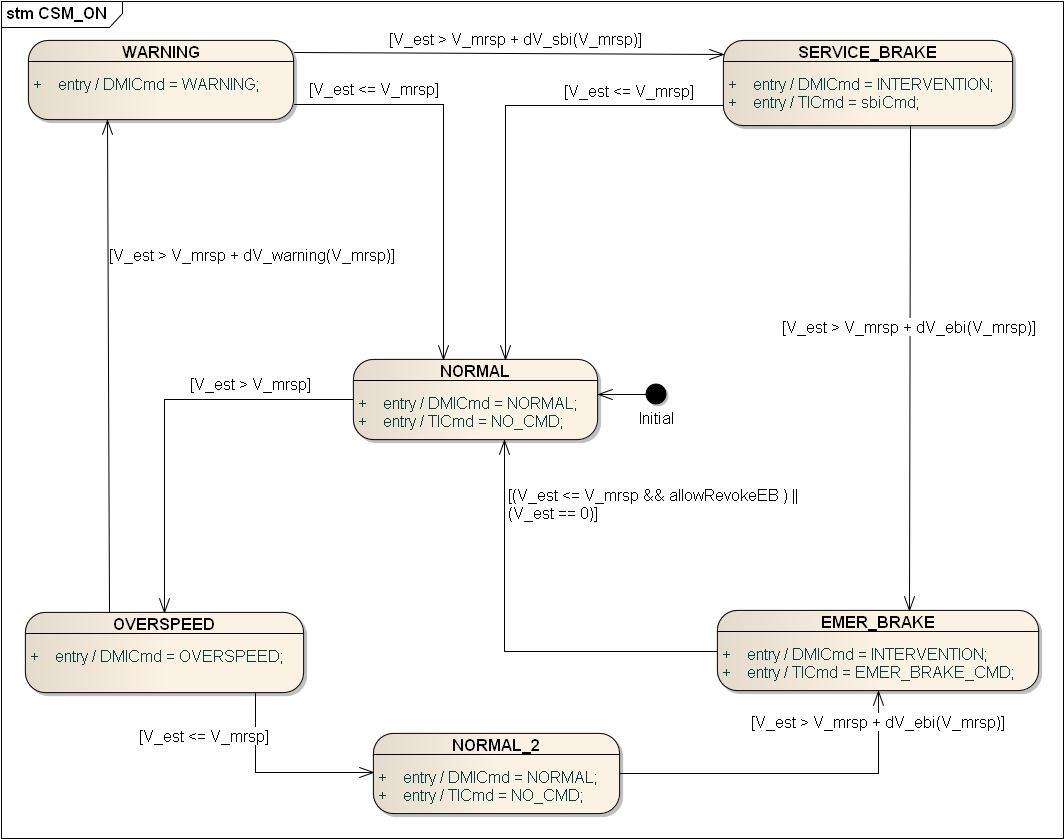
\includegraphics[width=1.3\textwidth]{CSM_ON_ADDITIONAL_STATE_FAILURE.png}
%%\vspace*{-35mm}
%%\end{center}
\caption{Faulty SUT -- Example~2.}
 \label{fig:addstatefail}
 \end{figure}





%-----------------------------------------------------------------------
\subsection{Example 3}\label{sec:example3}

Suppose that the implementation has an additional  control state $\text{NORMAL\_2}$ as
shown in the mutant in Figure~\ref{fig:mutant3}. When the SUT is in the control state $\text{Warning} $ and inputs satisfy $\vest\le \vmax$, the SUT's state machine transits to the new basic state  
$\text{NORMAL\_2}$. For this control state, there is only one outgoing transition in SysML whose guard condition is $ \vest > \vmax + dV_{\text {warning}}$, and target control state is $\text {Warning}$.
%As a consequence, the SUT fails to issue warnings and to trigger service brake intervention, after having entered $\text{NORMAL\_2}$; only the emergency brake intervention condition is handled correctly. The SUT failure remains hidden until a transition sequence from {\sf NORMAL} to {\sf OVERSPEED} and back to {\sf NORMAL} should be performed. 
Note that the introduction of this additional basic state in the SUT's SysML state machine leads to a DFSM abstraction that has {\it two} more states than the DFSM abstraction of the original model, because basic states {\sf NORMAL} and {\sf OVERSPEED} are no longer equivalent, and {\sf NORMAL\_2} is non-equivalent to any of the other states.


Assuming again the case $\sbz=1$ and applying $\text{TEST\_SUITE}_{\sbz=1}$ introduced in Section~\ref{sec:completesuites}, this failure will be uncovered, for example, by test case
\footnotesize
\begin{eqnarray*}
\iota & = & \vec c_4.\vec c_1.\vec c_3 
\\ & = & (\vest=125,\vmax=120,\areb=1).(60,90,0).(152,150,0)
\end{eqnarray*}
\normalsize
On the model $STS$, this input will trigger output sequence
$$
(\dmicmd=3,\ticmd=0).(0,0).(2,0)
$$
whereas output sequence
$$
(\dmicmd=3,\ticmd=0).(0,0).(0,0)
$$
will be triggered by $\iota$, when applied to $STS'$ representing the SUT. 

Observe that this SUT failure would not be uncovered by every ordinary transition coverage test strategy based on SysML state machine model. Transition coverage would be achieved, for example, by the test procedure TP-002 in Section~\ref{sec:conventionaltests}
%\begin{eqnarray*}
%\text{TC\_TEST\_SUITE} & = & \{ \vec c_3.\vec c_1. \vec c_3.\vec c_4.\vec c_1.\vec c_4.\vec c_5.\vec c_1.\vec c_5.\vec c_6.\vec c_2.\vec c_6.\vec c_2.\vec c_3.\vec c_5.\vec c_1.\vec c_4.\vec c_6.\vec c_2.\vec c_3.\vec c_6\}  
%\end{eqnarray*}
which fail to uncover the violation of I/O-equivalence.

 

 \begin{figure}
 \hspace*{-10mm}
%% \begin{center}
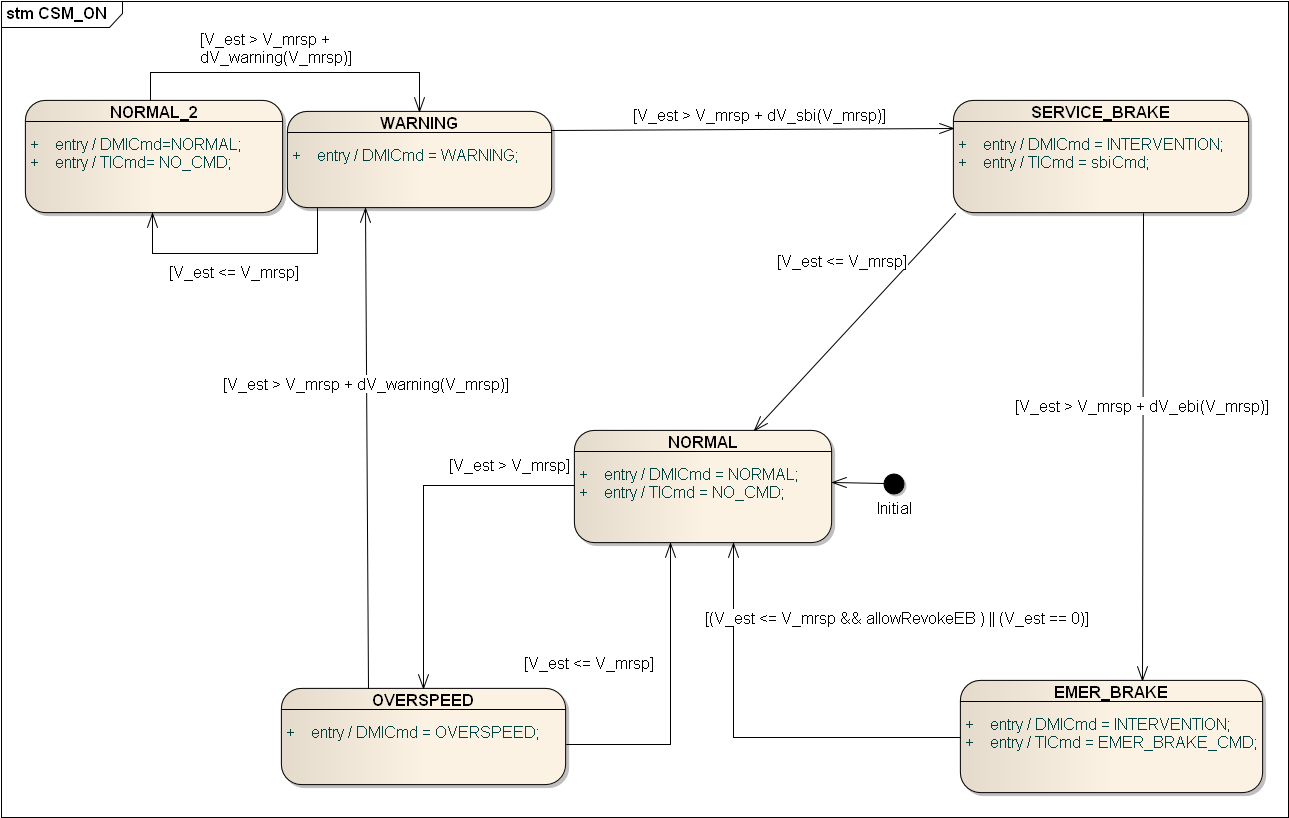
\includegraphics[width=1.2\textwidth]{CSM_ON_mutant_3.png}
%%\vspace*{-35mm}
%%\end{center}
\caption{Faulty SUT -- Example~3.}
 \label{fig:mutant3}
 \end{figure}

 

 

% =======================================================================
\section{Heuristics for Constructing IECP Refinements}\label{sec:refineheuristics}

\subsection{IECP Refinements for the CSM}\label{sec:iecprefine}

The definition of IECP refinements given in Section~\ref{sec:iecp} induces a construction 
mechanism based on propositions. This is applied to the CSM as follows.
\begin{enumerate}
\item Choose a new proposition $\gamma$ over free variables from $I$.
\item Strengthen each proposition $\Phi_k,\ k= 1,\dots,6$ defining an IEC   by
\begin{eqnarray*}
\Phi_{k,+}^I & \equiv & \Phi_k\wedge \gamma
\\
\Phi_{k,-}^I & \equiv & \Phi_k\wedge \neg\gamma
\end{eqnarray*}

\item Specify the refinement  by 
\begin{eqnarray*}
{\cal I}_2 & = & \{ X_{k,+},X_{k,-}~|~k = 1,\dots,6  \}
\\
X_{k,+} & = & \{\vec c\in D_I~|~\Phi_{k,+}[\vec c/(\vest,\vmax,\areb)]\} 
\\
X_{k,-} & = & \{\vec c\in D_I~|~\Phi_{k,-}[\vec c/(\vest,\vmax,\areb)]\} 
\end{eqnarray*}


\item Refine the old input alphabet by adding input vectors for each new $X_{k,+}, X_{k,-}$ which does not have a representative in the old alphabet.
\end{enumerate}


Refinements of the original IECP are needed, for example, when it is suspected that the SUT implements so-called {\it trapdoors}~\cite{libBinder2000}: these are transitions whose trigger conditions are refinements $\varphi_{q,i}^I\wedge \gamma$ of trigger conditions  $\varphi_{q,i}^I$ in the original model. The SUT behaviour conforms to the associated  model transition for inputs satisfying $\varphi_{q,i}^I\wedge \neg\gamma$, but shows erroneous behaviour for inputs satisfying  $\varphi_{q,i}^I\wedge \gamma$. Trapdoors may occur in transitions from quiescent to quiescent, and in transitions from quiescent to transient states. In the subsequent sections this and other motivations for introducing refinements are discussed.


% ----------------------------------------------------------------------------------------
\subsection{Overview of the Refinement Concept}
In this section we present and discuss a heuristic for constructing IECP refinements
resulting in larger fault domains that are well-justified from the perspective of 
standards related to safety-critical systems development in the avionic, automotive, and railway domains~\cite{do178b,DO178C,ISO26262-8,CENELEC50128}.


  

Our heuristic involves the following refinement steps, and we suggest to apply these in the order presented here.
\begin{enumerate}
\item Requirements-based IECP refinement
\item Boundary value IECP refinement
\item IECP refinement by sub-paving
\end{enumerate}

% --------------------------------------------------------------------
\subsection{Requirements-based IECP Refinement}

% --------------------------------------------------------------------
\subsubsection{Requirements-related Case Distinctions}

In Section~\ref{sec:transientinputcond} we introduced the transient state input 
conditions $\varphi_{q,i}^I$.
Intuitively speaking, each of these conditions, when feasible and applied in quiescent state class $q$, triggers a well-defined behaviour, namely the transformation of internal state and outputs performed by the transition from transient state class $B_i$ to its quiescent successor state class $A_i$. Since this transformation is constant (it only depends on $B_i$), it reflects one system requirement or a part of it. As a consequence, any disjunction occurring in such a 
condition $\varphi_{q,i}^I$ reflects a case distinction for the same requirement.

\begin{example}
Condition
$$
\varphi_{0,1}^I(V) \equiv \vmax < \vest \wedge \vest \le \vmax + \dvw(\vmax)
$$
reflects the pre-condition for requirement REQ-3.13.10.3.3.t2 (see Table~\ref{tab:five}), concerning the transition from {\sf NORMAL} state to {\sf OVERSPEED} state in the SysML state machine, with  activation of the overspeed indication at the driver machine interface. $\varphi_{0,1}^I(V)$ is applied in $A_0$, and triggers a transition into $B_1$ from where the overspeed indication is activated and the system stabilises again in $A_1$.
Expanding $\dvw(\vmax)$, we get
\begin{eqnarray*}
\varphi_{0,1}^I(V) &\equiv& \vmax < \vest \wedge {}
\\ & & ((\vmax \le 110 \wedge   \vest \le \vmax +4) \vee {}
\\ & & \ \ (110<\vmax \le 140  \wedge \vest \le \frac{31}{30}\vmax +\frac{1}{3} ) \vee {}
\\ & & \ \ (140<\vmax \wedge  \vest \le \vmax +5))
\end{eqnarray*}
The disjunction inside the second conjunct covers the three case distinctions for transiting into {\sf OVERSPEED} (see definition of $\dvw(\vmax)$ in Equation~(\ref{eq:dvw})).
\xbox
\end{example}

Similarly, the quiescent state conditions $\varphi_i^I(I) = \varphi_{i,i}^I(I)$ specify stability requirements regarding input changes that will not lead to any new system reaction, so disjunctions in $\varphi_{i,i}^I(I)$ represent case distinctions of these stability requirements.
\begin{example}
Condition
$$
\varphi_4^I(V) \equiv  \varphi_{4,4}^I(V)   \equiv    (0 < \vest   \wedge \areb=0) \vee (\vmax < \vest  \wedge \areb=1)
$$
describes the stability condition when in SysML state machine state {\sf EMER\_BRAKE}. There are two cases to consider.
\begin{enumerate}
\item When the emergency brake command may only be revoked after the train has come to a standstill 
(case $\areb=0$),  any input condition satisfying $0 < \vest$ is a stability condition when in basic state {\sf EMER\_BRAKE}.

\item When the emergency brake command may already be revoked as soon as $\vest \leq \vmax$
(case $\areb=1$), any input condition satisfying $\vmax < \vest$ is a stability condition when in basic state {\sf EMER\_BRAKE}.
\end{enumerate}
\xbox
\end{example}

Standards for safety-relevant systems always demand that requirements should be completely covered by tests (see, e.g.,\cite[6.4.4]{DO178C}). Therefore it is advisable to refine the IECP in such a way, that the extended input alphabet resulting from this refinement covers all requirements-related case distinctions.





% --------------------------------------------------------------------
\subsubsection{Construction of the Requirements-based IECP Refinement}

The mechanisable construction of the requirements-based IECP refinement is performed
for the CSM  as follows.
\begin{enumerate}
\item Transform each $\varphi_{q,i}^I$ and each $\varphi_{i,i}^I$ into disjunctive normal form (DNF). This results in disjuncts $\varphi_{q,i,h}^I$, such that
$$
\varphi_{q,i}^I \equiv \bigvee_j \varphi_{q,i,h}^I
$$
Define index set $I_q$ as the set of all pairs $(i,h)$ where $\varphi_{q,i,h}^I$ is a disjunct in the DNF of $\varphi_{q,i}^I$.


\item Drop infeasible disjuncts. This can be performed by means of an SMT solver determining for each disjunct whether it has at least one solution.

\item Refine the $\Phi_k,\ k=1,\dots,6$ specifying the IECP of the CSM as 
described in Section~\ref{sec:csmiecpxxx} to propositions
$$
      \Phi_{k,(j_0,h_0),\dots,(j_4,h_4)} \equiv \bigwedge_{q=0}^4 \varphi_{q,j_q,h_q}^I
$$
where $(j_q,h_q)\in I_q,\ q = 0,\dots,4$.


\item Create IECs in analogy to the rules given in Section~\ref{sec:iecp}, but this time using feasible solutions $\Phi_{k,(j_0,h_0),\dots,(j_4,h_4)}$:
$$
X_{k,(j_0,h_0),\dots,(j_4,h_4)} = \{\vec c\in D_I~|~\Phi_{k,(j_0,h_0),\dots,(j_4,h_4)}[\vec c/(\vest,\vmax,\areb)]\}
$$

\item Determine the $X_{k,(j_0,h_0),\dots,(j_4,h_4)}$ that are already represented by the existing members $\vec c$  of the old alphabet.

\item  For each of the remaining $X_{k,(j_0,h_0),\dots,(j_4,h_4)}$, select a new member for the new, extended input alphabet by letting a constraint solver find a solution $\vec c$ for 
$$\Phi_{k,(j_0,h_0),\dots,(j_4,h_4)}[\vec c/(\vest,\vmax,\areb)]$$

\end{enumerate}

\begin{example}
For the CSM, the requirements-based IECP-refinement leads to the following disjuncts $\varphi_{q,i,j}^I$.
%\footnotesize
\begin{eqnarray*}
\varphi_{0,0,0}^I & \equiv & \varphi_0^I(V)  \equiv \vest \le \vmax
\\
\varphi_{1,1,0}^I & \equiv & \vmax \le 110 \wedge   \vmax <  \vest \le \vmax +4
\\
\varphi_{1,1,1}^I & \equiv & 110<\vmax  \le 140  \wedge \vmax < \vest \le \frac{31}{30}\vmax +\frac{1}{3}
\\
\varphi_{1,1,2}^I & \equiv & 140<\vmax \wedge  \vmax < \vest \le \vmax +5
\\
\varphi_{2,2,0}^I & \equiv &  \vmax \le 110 \wedge  \vmax < \vest \le \vmax + 5.5
\\
\varphi_{2,2,1}^I & \equiv &  110 <\vmax  \le 210 \wedge 
\vmax < \vest \le\frac{209}{200}\vmax +\frac{55}{100}
\\
\varphi_{2,2,2}^I & \equiv & 210 < \vmax  \wedge  \vmax <  \vest \le\vmax + 10
\\
\varphi_{3,3,0}^I & \equiv &   \vmax \le 110 \wedge \vmax < \vest \le  \vmax + 7.5
\\
\varphi_{3,3,1}^I & \equiv &   110<\vmax  \le 210 \wedge  \vmax < \vest \le  \frac{43}{40}\vmax -\frac{3}{4}
\\
\varphi_{3,3,2}^I & \equiv &  210<\vmax   \wedge  \vmax < \vest \le  \vmax +15
\\ 
\varphi_{4,4,0}^I  & \equiv &  0 < \vest \le \vmax   \wedge \areb=0
\\ 
\varphi_{4,4,1}^I  & \equiv &  \vmax < \vest  
\\
\varphi_{0,1,0}^I &\equiv& \vmax \le 110 \wedge   \vmax < \vest \le \vmax +4
\\
\varphi_{0,1,1}^I &\equiv& 110<\vmax \le 140  \wedge \vmax < \vest \le \frac{31}{30}\vmax +\frac{1}{3} 
\\  
\varphi_{0,1,2}^I &\equiv& 140<\vmax \wedge  \vmax < \vest \le \vmax +5
\\
\varphi_{0,2,0}^I &\equiv& \vmax \le 110 \wedge \vmax +4 < \vest \le \vmax + 5.5
\\
\varphi_{0,2,1}^I &\equiv&  110 <\vmax  \le 140 \wedge \frac{31}{30}\vmax +\frac{1}{3} < \vest \le\frac{209}{200}\vmax +\frac{55}{100}
\\
\varphi_{0,2,2}^I &\equiv&  140 < \vmax \le 210 \wedge \vmax +5 < \vest \le\frac{209}{200}\vmax +\frac{55}{100}
\\
\varphi_{0,2,3}^I &\equiv&  210 < \vmax  \wedge  \vmax +5 < \vest \le\vmax + 10
\\
\varphi_{0,3,0}^I &\equiv& \vmax \le 110 \wedge \vmax + 5.5 < \vest \le  \vmax + 7.5
\\
\varphi_{0,3,1}^I &\equiv& 110<\vmax \le 210 \wedge \frac{209}{200}\vmax +\frac{55}{100}< \vest \le  \frac{43}{40}\vmax -\frac{3}{4}
\\
\varphi_{0,3,2}^I &\equiv& 210<\vmax   \wedge \vmax +10 < \vest \le  \vmax +15
\\
\varphi_{0,4,0}^I &\equiv& \vmax \le 110 \wedge \vmax + 7.5 < \vest
\\
\varphi_{0,4,1}^I &\equiv& 110<\vmax \le 210 \wedge  \frac{43}{40}\vmax -\frac{3}{4}< \vest
\\
\varphi_{0,4,2}^I &\equiv& 210<\vmax   \wedge \vmax +15 < \vest
\end{eqnarray*}
%\normalsize

%\footnotesize
\begin{eqnarray*}
\varphi_{1,2,i}^I &\equiv& \varphi_{0,2,i}^I, \ i = 0,1,2,3
\\  
\varphi_{1,3,i}^I &\equiv& \varphi_{0,3,i}^I, \ i = 0,1,2
\\
\varphi_{1,4,i}^I &\equiv& \varphi_{0,4,i}^I, \ i = 0,1,2
\\
\varphi_{2,3,i}^I &\equiv& \varphi_{0,3,i}^I \ i = 0,1,2
\\ 
\varphi_{2,4,i}^I &\equiv& \varphi_{0,4,i}^I \ i = 0,1,2
\\
\varphi_{3,4,i}^I &\equiv& \varphi_{0,4,i}^I \ i = 0,1,2
\\
\varphi_{1,0,0}^I &\equiv& \varphi_{1,0} \equiv \vest \le \vmax  
\\
\varphi_{2,0,0}^I &\equiv& \varphi_{1,0,0}^I  
\\
\varphi_{3,0,0}^I &\equiv& \varphi_{1,0,0}^I  
\\
\varphi_{4,0,0}^I &\equiv& \vest = 0 
\\
\varphi_{4,0,1}^I &\equiv& 0 < \vest \le \vmax \wedge \areb = 1
\end{eqnarray*}
%\normalsize

This leads to the following refined predicates $\Phi_{i_j}$.
%\footnotesize
\begin{eqnarray*}
\Phi_{1_0} & \equiv & \varphi_{0,0,0}^I \wedge \varphi_{1,0,0}^I \wedge \varphi_{2,0,0}^I \wedge \varphi_{3,0,0}^I \wedge \varphi_{4,4,0}^I
\\ & \equiv & \varphi_{0,0,0}^I \wedge \varphi_{4,4,0}^I
\\ & \equiv & 0 < \vest \le \vmax \wedge \areb = 0
\\
\Phi_{2_0} & \equiv & \varphi_{0,0,0}^I \wedge \varphi_{1,0,0}^I \wedge \varphi_{2,0,0}^I \wedge \varphi_{3,0,0}^I \wedge \varphi_{4,0,0}^I
\\ & \equiv & \varphi_{4,0,0}^I
\\ & \equiv & \vest = 0 % \vee (\vest \le \vmax \wedge \areb = 1)
\\
\Phi_{2_1} & \equiv & \varphi_{0,0,0}^I \wedge \varphi_{1,0,0}^I \wedge \varphi_{2,0,0}^I \wedge \varphi_{3,0,0}^I \wedge \varphi_{4,0,1}^I
\\ & \equiv & \varphi_{4,0,1}^I
\\ & \equiv & 0 < \vest \le \vmax \wedge \areb = 1
\\
\Phi_{3_0} & \equiv & \varphi_{0,1,0}^I \wedge \varphi_{1,1,0}^I \wedge  \varphi_{2,2,0}^I \wedge \varphi_{3,3,0}^I \wedge \varphi_{4,4,1}^I 
\\ & \equiv &  \vmax \le 110 \wedge   \vmax <  \vest \le \vmax +4  
\\
\Phi_{3_1} & \equiv &  \varphi_{0,1,1}^I \wedge \varphi_{1,1,1}^I \wedge  \varphi_{2,2,1}^I \wedge \varphi_{3,3,1}^I \wedge \varphi_{4,4,1}^I 
\\ & \equiv & 110<\vmax \le 140  \wedge \vmax < \vest \le \frac{31}{30}\vmax +\frac{1}{3}
\\
\Phi_{3_2} & \equiv &  \varphi_{0,1,2}^I \wedge \varphi_{1,1,2}^I \wedge  \varphi_{2,2,1}^I \wedge \varphi_{3,3,1}^I \wedge \varphi_{4,4,1}^I 
\\ & \equiv & 140 < \vmax \le 210 \wedge \vmax <  \vest \le\vmax + 5 
\end{eqnarray*}
%\normalsize

%\footnotesize
\begin{eqnarray*}
\Phi_{3_3} & \equiv &  \varphi_{0,1,2}^I \wedge \varphi_{1,1,2}^I \wedge  \varphi_{2,2,2}^I \wedge \varphi_{3,3,2}^I \wedge \varphi_{4,4,1}^I 
\\ & \equiv & 210 < \vmax <  \vest \le\vmax + 5 
\\
\Phi_{4_0} & \equiv &  \varphi_{0,2,0}^I \wedge \varphi_{1,2,0}^I \wedge \varphi_{2,2,0}^I \wedge  \varphi_{3,3,0}^I \wedge \varphi_{4,4,1}^I 
\\ & \equiv & \vmax \le 110 \wedge \vmax +4 < \vest \le \vmax + 5.5 
\\
\Phi_{4_1} & \equiv &  \varphi_{0,2,1}^I \wedge \varphi_{1,2,1}^I \wedge \varphi_{2,2,1}^I \wedge  \varphi_{3,3,1}^I \wedge \varphi_{4,4,1}^I 
\\ & \equiv & 110 <\vmax  \le 140 \wedge \frac{31}{30}\vmax +\frac{1}{3} < \vest \le\frac{209}{200}\vmax +\frac{55}{100}
\\
\Phi_{4_2} & \equiv &  \varphi_{0,2,2}^I \wedge \varphi_{1,2,2}^I \wedge \varphi_{2,2,1}^I \wedge  \varphi_{3,3,1}^I \wedge \varphi_{4,4,1}^I 
\\ & \equiv & 140 < \vmax \le 210 \wedge \vmax +5 < \vest \le\frac{209}{200}\vmax +\frac{55}{100}
\\
\Phi_{4_3} & \equiv &  \varphi_{0,2,3}^I \wedge \varphi_{1,2,3}^I \wedge \varphi_{2,2,2}^I \wedge  \varphi_{3,3,2}^I \wedge \varphi_{4,4,1}^I 
\\ & \equiv & 210 < \vmax  \wedge  \vmax +5 < \vest \le\vmax + 10 
\\
\Phi_{5_0} & \equiv &  \varphi_{0,3,0}^I \wedge \varphi_{1,3,0}^I \wedge \varphi_{2,3,0}^I \wedge  \varphi_{3,3,0}^I \wedge \varphi_{4,4,1}^I 
\\ & \equiv & \vmax \le 110 \wedge \vmax + 5.5 < \vest \le  \vmax + 7.5 
\\
\Phi_{5_1} & \equiv &  \varphi_{0,3,1}^I \wedge \varphi_{1,3,1}^I \wedge \varphi_{2,3,1}^I \wedge  \varphi_{3,3,1}^I \wedge \varphi_{4,4,1}^I 
\\ & \equiv & 110<\vmax \le 210 \wedge \frac{209}{200}\vmax +\frac{55}{100}< \vest \le  \frac{43}{40}\vmax -\frac{3}{4}
\\
\Phi_{5_2} & \equiv &  \varphi_{0,3,2}^I \wedge \varphi_{1,3,2}^I \wedge \varphi_{2,3,2}^I \wedge  \varphi_{3,3,2}^I \wedge \varphi_{4,4,1}^I 
\\ & \equiv & 210<\vmax   \wedge \vmax +10 < \vest \le  \vmax +15 
\\
\Phi_{6_0} & \equiv &  \varphi_{0,4,0}^I \wedge \varphi_{1,4,0}^I \wedge \varphi_{2,4,0}^I \wedge  \varphi_{3,4,0}^I \wedge \varphi_{4,4,1}^I 
\\ & \equiv & \vmax \le 110 \wedge \vmax + 7.5 < \vest 
\\
\Phi_{6_1} & \equiv &  \varphi_{0,4,1}^I \wedge \varphi_{1,4,1}^I \wedge \varphi_{2,4,1}^I \wedge  \varphi_{3,4,1}^I \wedge \varphi_{4,4,1}^I 
\\ & \equiv & 110<\vmax \le 210 \wedge  \frac{43}{40}\vmax -\frac{3}{4}< \vest 
\\
\Phi_{6_2} & \equiv &  \varphi_{0,4,2}^I \wedge \varphi_{1,4,2}^I \wedge \varphi_{2,4,2}^I \wedge  \varphi_{3,4,2}^I \wedge \varphi_{4,4,1}^I 
\\ & \equiv & 210<\vmax   \wedge \vmax +15 < \vest 
\end{eqnarray*}
%\normalsize
%===================================================================

\begin{table}[htdp]
\caption{Extended input alphabet ${{\cal A}}'_I$ satisfying  ${\cal A}_I\subseteq {{\cal A}}'_I$.}
\begin{center}
\begin{tabular}{|c||c|c|c||c|c|}
\hline\hline
$\vec c_i$&$\vmax$&$\vest$&$\areb$&$X_i$ & $X_{i_j}$ \\\hline\hline
$\vec c_1$&90&60&0&$X_1$&$X_{1_0}$ \\
$\vec c_2$&90&60&1&$ X_2$ &$X_{2_1}$ \\
$\vec c_3$&150&152&0&$X_3$ &$X_{3_2}$ \\
$\vec c_4$&120&125&1&$X_4$&$X_{4_1}$ \\
$\vec c_{5}$&60&66&0&$X_5$&$X_{5_0}$ \\
$\vec c_{6}$&230&260&1&$X_6$&$X_{6_2}$\\\hline
% 
$\vec c_{7}$&90&0&1& $ X_2$  &$X_{2_0}$ \\
%
$\vec c_{8}$&90&93&0&$X_3$ &$X_{3_0}$ \\
$\vec c_{9}$&112&115&1&$X_3$&$X_{3_1}$ \\
$\vec c_{10}$&211&212&0&$X_3$ &$X_{3_3}$ \\
%
$\vec c_{11}$&90&95&1&$X_4$&$X_{4_0}$ \\
$\vec c_{12}$&150&156&0&$X_4$&$X_{4_2}$ \\
$\vec c_{13}$&220&226&1&$X_4$&$X_{4_3}$ \\
%
$\vec c_{14}$&205&215&0&$X_5$&$X_{5_1}$ \\
$\vec c_{15}$&230&244&1&$X_5$&$X_{5_2}$ \\
%
$\vec c_{16}$&55&100&0&$X_6$&$X_{6_0}$ \\
$\vec c_{17}$&200&215&1&$X_6$&$X_{6_1}$ 
\\\hline\hline
\end{tabular}
%\normalsize
\end{center}
\label{tab:inputalphabetreqref}
\end{table}

From the refined predicates additional members of the input alphabet are selected. This results
in a new alphabet as the one shown in Table~\ref{tab:inputalphabetreqref}.

The resulting test suite comprises the test cases of the old suite plus additional cases, 
the new test suite can be expressed as an extension of the old one.
Since $(A\cup B)^3=A^3\cup A^2.B\cup A.B.(A\cup B)\cup B.(A\cup B)^2$, for any subsets $A,B$ of the input alphabet, the old input alphabet with set $A=\{c_1,\dots,c_6\}$, and the new alphabet values 
contained in $B=\{c_7,\dots,c_{17}\}$   result in the following test suite.
\footnotesize
\begin{eqnarray*}
{\text{TEST\_SUITE}_{\sbz=1}}' & = & 
\{\vec c_i.\vec c_j.\vec c_k.\vec c_3~|~i,j,k=1,\dots,17\} \cup{}
\\ & &
\{\vec c_j.\vec c_i.\vec c_k.\vec c_h.\vec c_3~|~h,i,k=1,\dots,17,j = 4,5,6 \} \cup {}
\\
& = &
\{\vec c_i.\vec c_j.\vec c_k.\vec c_3~|~i,j,k=1,\dots,6\} \cup{}
\\ & &
\{\vec c_j.\vec c_i.\vec c_k.\vec c_h.\vec c_3~|~h,i,k=1,\dots,6,j = 4,5,6 \} \cup {}
\\ & & 
\{\vec c_i.\vec c_j.\vec c_k.\vec c_3~|~i,j=1,\dots,6, k=7,\dots,17\} \cup{}
\\ & &
\{\vec c_i.\vec c_k.\vec c_j.\vec c_3~|~i=1,\dots,6, j=1,\dots,17, k=7,\dots,17\} \cup{}
\\ & &
\{\vec c_k.\vec c_i.\vec c_j.\vec c_3~|~i,j=1,\dots,17, k=7,\dots,17\} \cup{}
\\ & &
\{\vec c_j.\vec c_i.\vec c_h.\vec c_k.\vec c_3~|~i,h=1,\dots,6, k=7,\dots,17,j = 4,5,6 \} \cup {}
\\ & & 
\{\vec c_j.\vec c_i.\vec c_k.\vec c_h.\vec c_3~|~i=1,\dots,6, h=1,\dots,17,  k=7,\dots,17,j = 4,5,6 \} \cup {}
\\ & & 
\{\vec c_j.\vec c_k.\vec c_i.\vec c_h.\vec c_3~|~i,h=1,\dots,17, k=7,\dots,17, j = 4,5,6\}
\end{eqnarray*}
\xbox
\end{example}
% ........................................................................
\subsubsection{Discussion}

The requirements-based IECP refinement ensures that all case distinctions of requirements are tested. As a consequence, all SUT failures will be detected, where in a certain SUT state all inputs that should trigger the reaction for a given requirements sub-case are handled incorrectly. Compared to the original IECP, this is a considerable improvement, because the original IECP is only guaranteed to detect failures if {\it all} sub-cases of a requirement are incorrectly handled by the SUT in a certain state.

Just as for the original IECP, however, the requirements-based IECP refinement relies on the SUT implementing all control decisions, that is, all guard conditions specified in the original SysML state machine, correctly. Failures are only allowed in the actions setting outputs and internal states. This is of considerable value if SUT code is generated semi-automatically.  A qualified code-frame generator, for example, might derive a control procedure from the state machine model, so that all control states, guard conditions, and state machine transitions are generated with high reliability by the tool. However, the driver software implementing access to the hardware output interfaces -- in our example the DMI and the train interface acting on the brakes -- may have been implemented in a manual way, so that some actions will show erroneous behaviour in certain states of the SUT. 

For other development scenarios, in particular, when the SUT code has been developed from the requirements in manual way, the test strength of the requirements-based IECP refinement is still insufficient, because SUT failures in the handling of guard conditions are just as likely as failures in the action implementations. These failure scenarios will be considered in the next refinements.


% --------------------------------------------------------------------
\subsection{Boundary Value IECP Refinement}
Let ${\cal I}_2=\{X_{1_0},X_{2_0},X_{2_1},\dots, X_{6_2}\}$ be the input equivalence class partitioning containing the $17$ input equivalence classes constructed above by $\Phi_{i_j}$. Extend the old input alphabet to a new input alphabet which includes input vectors of the boundary of each $X_{i_j}$. Then the new input alphabet (see Table~\ref{tab:inputalphabetreqrefboundary}) contains $31$ inputs more then the old one, and the new test suite contains $4\cdot 48^3=442368$ test cases, $4\cdot 48^3- 4\cdot 17^3=442368-19652=422716$ test cases more.  

Since the CSM code does not depend on dealt-time conditions, this is still an acceptable number of software tests. For hardware-in-the-loop tests, when timing constraints of the target hardware and the operational environment have to be considered, however, it would be too time-consuming to execute them all. A well-justified reduction heuristic in this case is to drop the tests of certain boundary values for states where these boundaries are of no relevance. 


 
%=========================
The following refined predicates $\Phi_{i_j,k}$ contain the separate boundary conditions. 
%\footnotesize
\begin{eqnarray*}
\Phi_{1_0,0} & \equiv &  0 < \vest < \vmax \wedge \areb = 0
\\
\Phi_{1_0,1} & \equiv & 
 0 < \vest = \vmax \wedge \areb = 0
\\
\Phi_{2_0} & \equiv & \vest = 0 % \vee (\vest \le \vmax \wedge \areb = 1)
\\
\Phi_{2_1,0} & \equiv &  0 < \vest < \vmax \wedge \areb = 1
\\
\Phi_{2_1,1} & \equiv &  \vest = \vmax \wedge \areb = 1
\\
\Phi_{3_0,0} & \equiv &  \vmax < 110 \wedge   \vmax <  \vest < \vmax +4  
\\
\Phi_{3_0,1} & \equiv &  \vmax = 110 \wedge   \vmax <  \vest < \vmax +4  
\\
\Phi_{3_0,2} & \equiv &  \vmax < 110 \wedge     \vest = \vmax +4  
\\
\Phi_{3_0,3} & \equiv &  \vmax = 110 \wedge    \vest = \vmax +4  
\\
\Phi_{3_1,0} & \equiv &   110<\vmax < 140  \wedge \vmax < \vest < \frac{31}{30}\vmax +\frac{1}{3}
\\
\Phi_{3_1,1} & \equiv &   \vmax = 140  \wedge \vmax < \vest < \frac{31}{30}\vmax +\frac{1}{3}
\\
\Phi_{3_1,2} & \equiv &   110<\vmax < 140  \wedge  \vest = \frac{31}{30}\vmax +\frac{1}{3}
\\
\Phi_{3_1,3} & \equiv &   \vmax = 140  \wedge \vmax < \vest = \frac{31}{30}\vmax +\frac{1}{3}
\\
\Phi_{3_2,0} & \equiv &   140 < \vmax < 210 \wedge \vmax <  \vest <\vmax + 5
\\
\Phi_{3_2,1} & \equiv &    \vmax = 210 \wedge \vmax <  \vest <\vmax + 5
\\
\Phi_{3_2,2} & \equiv &   140 < \vmax < 210 \wedge   \vest =\vmax + 5
\\
\Phi_{3_2,3} & \equiv &    \vmax = 210 \wedge   \vest =\vmax + 5 
\\
\Phi_{3_3,0} & \equiv &   210 < \vmax <  \vest <\vmax + 5 
\\
\Phi_{3_3,1} & \equiv &   210 < \vmax <  \vest =\vmax + 5 
\\
\Phi_{4_0,0} & \equiv &   \vmax < 110 \wedge \vmax +4 < \vest < \vmax + 5.5 
\\
\Phi_{4_0,1} & \equiv &   \vmax = 110 \wedge \vmax +4 < \vest < \vmax + 5.5 
\\
\Phi_{4_0,2} & \equiv &   \vmax < 110 \wedge  \vest = \vmax + 5.5 
\\
\Phi_{4_0,3} & \equiv &   \vmax = 110 \wedge  \vest =\vmax + 5.5 
\\
\Phi_{4_1,0} & \equiv &   110 <\vmax  < 140 \wedge \frac{31}{30}\vmax +\frac{1}{3} < \vest <\frac{209}{200}\vmax +\frac{55}{100}
\\
\Phi_{4_1,1} & \equiv &   \vmax  = 140 \wedge \frac{31}{30}\vmax +\frac{1}{3} < \vest <\frac{209}{200}\vmax +\frac{55}{100}
\\
\Phi_{4_1,2} & \equiv &   110 <\vmax  < 140 \wedge  \vest =\frac{209}{200}\vmax +\frac{55}{100}
\\
\Phi_{4_1,3} & \equiv &   \vmax  = 140 \wedge \vest =\frac{209}{200}\vmax +\frac{55}{100}
\\
\Phi_{4_2,0} & \equiv & 140 < \vmax < 210 \wedge \vmax +5 < \vest <\frac{209}{200}\vmax +\frac{55}{100}
\\
\Phi_{4_2,1} & \equiv &  \vmax = 210 \wedge \vmax +5 < \vest <\frac{209}{200}\vmax +\frac{55}{100}
\\
\Phi_{4_2,2} & \equiv & 140 < \vmax < 210 \wedge  \vest= \frac{209}{200}\vmax +\frac{55}{100}
\\
\Phi_{4_2,3} & \equiv & \vmax = 210 \wedge  \vest= \frac{209}{200}\vmax +\frac{55}{100}
\\
\Phi_{4_3,0} & \equiv &  210 < \vmax  \wedge  \vmax +5 < \vest <\vmax + 10 
\\
\Phi_{4_3,1} & \equiv &  210 < \vmax  \wedge   \vest =\vmax + 10 
\end{eqnarray*}

\begin{eqnarray*}
\Phi_{5_0,0} & \equiv &  \vmax < 110 \wedge \vmax + 5.5 < \vest < \vmax + 7.5 
\\
\Phi_{5_0,1} & \equiv &  \vmax = 110 \wedge \vmax + 5.5 < \vest <  \vmax + 7.5 
\\
\Phi_{5_0,2} & \equiv &  \vmax < 110 \wedge  \vest =  \vmax + 7.5 
\\
\Phi_{5_0,3} & \equiv &  \vmax = 110 \wedge  \vest =  \vmax + 7.5 
\\
\Phi_{5_1,0} & \equiv &   110<\vmax < 210 \wedge \frac{209}{200}\vmax +\frac{55}{100}< \vest <  \frac{43}{40}\vmax -\frac{3}{4}
\\
\Phi_{5_1,1} & \equiv &   \vmax =210 \wedge \frac{209}{200}\vmax +\frac{55}{100}< \vest <  \frac{43}{40}\vmax -\frac{3}{4}
\\
\Phi_{5_1,2} & \equiv &  110< \vmax < 210 \wedge \vest = \frac{43}{40}\vmax -\frac{3}{4}
\\
\Phi_{5_1,3} & \equiv &   \vmax = 210 \wedge \vest =  \frac{43}{40}\vmax -\frac{3}{4}
\\
\Phi_{5_2,0} & \equiv &   210<\vmax   \wedge \vmax +10 < \vest <  \vmax +15 
\\
\Phi_{5_2,1} & \equiv &   210<\vmax   \wedge  \vest =  \vmax +15 
\\
\Phi_{6_0,0} & \equiv & \vmax < 110 \wedge \vmax + 7.5 < \vest 
\\
\Phi_{6_0,1} & \equiv & \vmax = 110 \wedge \vmax + 7.5 < \vest 
\\
\Phi_{6_1,0} & \equiv &  110<\vmax < 210 \wedge  \frac{43}{40}\vmax -\frac{3}{4}< \vest 
\\
\Phi_{6_1,1} & \equiv &  \vmax = 210 \wedge  \frac{43}{40}\vmax -\frac{3}{4}< \vest 
\\
\Phi_{6_2} & \equiv &   210<\vmax   \wedge \vmax +15 < \vest 
\end{eqnarray*}
%\normalsize


\begin{table}[htdp]
\caption{Extended input alphabet ${{\cal A}}_I$ containing boundary values.}
\begin{center}
\scriptsize
\begin{tabular}{|c||c|c|c||c|c|}
\hline\hline
$\vec c_i$&$\vmax$&$\vest$&$\areb$&$X_i$ & $X_{i_j,k}$ \\\hline\hline
$\vec c_1$&90&60&0&$X_1$&$X_{1_0,0}$ \\
$\vec c_2$&90&60&1&$ X_2$ &$X_{2_1,0}$ \\
$\vec c_3$&150&152&0&$X_3$ &$X_{3_2,0}$ \\
$\vec c_4$&120&125&1&$X_4$&$X_{4_1,0}$ \\
$\vec c_{5}$&60&66&0&$X_5$&$X_{5_0,0}$ \\
$\vec c_{6}$&230&260&1&$X_6$&$X_{6_2}$\\\hline
% 
$\vec c_{7}$&90&0&1& $ X_2$  &$X_{2_0}$ \\
%
$\vec c_{8}$&90&93&0&$X_3$ &$X_{3_0,0}$ \\
$\vec c_{9}$&112&115&1&$X_3$&$X_{3_1,0}$ \\
$\vec c_{10}$&211&212&0&$X_3$ &$X_{3_3,0}$ \\
%
$\vec c_{11}$&90&95&1&$X_4$&$X_{4_0,0}$ \\
$\vec c_{12}$&150&156&0&$X_4$&$X_{4_2,0}$ \\
$\vec c_{13}$&220&226&1&$X_4$&$X_{4_3,0}$ \\
%
$\vec c_{14}$&205&215&0&$X_5$&$X_{5_1,0}$ \\
$\vec c_{15}$&230&244&1&$X_5$&$X_{5_2,0}$ \\
%
$\vec c_{16}$&55&100&0&$X_6$&$X_{6_0,0}$ \\
$\vec c_{17}$&200&215&1&$X_6$&$X_{6_1,0}$ 
\\\hline\hline
$\vec c_{18}$&90&90&0&$X_1$&$X_{1_0,1}$ \\
$\vec c_{19}$&90&90&1&$ X_2$ &$X_{2_1,1}$ \\
$\vec c_{20}$&110&113&0&$X_3$ &$X_{3_0,1}$ \\
$\vec c_{21}$&90&94&0&$X_3$ &$X_{3_0,2}$ \\
$\vec c_{22}$&110&114&0&$X_3$ &$X_{3_0,3}$ \\
$\vec c_{23}$&140&143&1&$X_3$&$X_{3_1,1}$ \\
$\vec c_{24}$&120&124,3&1&$X_3$&$X_{3_1,2}$ \\
$\vec c_{25}$&140&145&1&$X_3$&$X_{3_1,3}$ \\
$\vec c_{26}$&210&212&0&$X_3$ &$X_{3_2,1}$ \\
$\vec c_{27}$&150&155&0&$X_3$ &$X_{3_2,2}$ \\
$\vec c_{28}$&210&215&0&$X_3$ &$X_{3_2,3}$ \\
$\vec c_{29}$&211&216&0&$X_3$ &$X_{3_3,1}$ \\
$\vec c_{30}$&110&115&1&$X_4$&$X_{4_0,1}$ \\
$\vec c_{31}$&90&95,5&1&$X_4$&$X_{4_0,2}$ \\
$\vec c_{32}$&110&115,5&1&$X_4$&$X_{4_0,3}$ \\
$\vec c_{33}$&140&146&1&$X_4$&$X_{4_1,1}$ \\
$\vec c_{34}$&120&125,95&1&$X_4$&$X_{4_1,2}$ \\
$\vec c_{35}$&140&146,85&1&$X_4$&$X_{4_1,3}$ \\
$\vec c_{36}$&210&218&0&$X_4$&$X_{4_2,1}$ \\
$\vec c_{37}$&150&157,3&0&$X_4$&$X_{4_2,2}$ \\
$\vec c_{38}$&210&220&0&$X_4$&$X_{4_2,3}$ \\
$\vec c_{39}$&220&230&1&$X_4$&$X_{4_3,1}$ \\
$\vec c_{40}$&110&116&0&$X_5$&$X_{5_0,1}$ \\
$\vec c_{41}$&60&67,5&0&$X_5$&$X_{5_0,2}$ \\
$\vec c_{42}$&110&117,5&0&$X_5$&$X_{5_0,3}$ \\
$\vec c_{43}$&210&215&0&$X_5$&$X_{5_1,1}$ \\
$\vec c_{44}$&200&214,25&0&$X_5$&$X_{5_1,2}$ \\
$\vec c_{45}$&210&225&0&$X_5$&$X_{5_1,3}$ \\
$\vec c_{46}$&220&235&1&$X_5$&$X_{5_2,1}$ \\
$\vec c_{47}$&110&118&0&$X_6$&$X_{6_0,1}$ \\
$\vec c_{48}$&210&226&1&$X_6$&$X_{6_1,1}$ 
\\\hline\hline
\end{tabular}
\normalsize
\end{center}
\label{tab:inputalphabetreqrefboundary}
\end{table}


% --------------------------------------------------------------------
\subsection{IECP Refinement by Sub-paving}

After having considered all case distinctions related to requirements and all boundary value situations, further refinements are motivated by the possibility of trapdoors implemented in the SUT, so that erroneous behaviour is revealed in certain SUT states for unknown subsets of the input classes obtained so far by the previous two refinement steps.

In principle, trapdoors triggered by a subset containing an interval vector of the input domain with positive diameter can be detected by further refining the input classes using sub-paving, that is, by partitioning the input classes using intersections with interval vectors~\cite{jaulin2001}.
In absence of any hints concerning size and location of trapdoors inside the existing input classes,
there is no evidence, however, that this systematic partitioning will be more effective than just choosing additional uniformly distributed random values from each input class, in addition to the inputs systematically constructed in the previous steps. 




% --------------------------------------------------------------------
\subsection{Effects of IECP Refinements on W-Method Application}

Since  IECP refinements always increase the input alphabet, but do not refine the quiescent or transient state classes, previous test suites performed for a coarser alphabet can be re-used, if the following rules are applied.
\begin{enumerate}
\item The characterisation set $W$ remain unchanged by refinements, since it uniquely identifies states, and states are not refined by IECP refinements.

\item The state transition cover $STC$ is always {\it extended} in the following way.
\begin{itemize}
\item Whenever a quiescent state class is encountered for the first time during STC construction, all members of the alphabet are applied to the state.
\end{itemize}
Since this rule was already applied in the initial STC construction, the previous STC is always a subset of the new STC.
\end{enumerate}

Let $STC$, ${\cal A}_I$ denote the state transition cover and input alphabet associated with the old IECP, and let $STC'$, ${\cal A}_I'$ denote the ones associated with the refined IECP.
Providing that the previous IECP has already been completely tested using the W-Method with test suite ${\cal W}(STS)$, 
the additional test cases to be performed with the refined IECP are
\begin{eqnarray*}
{\cal W}'(STS) - {\cal W}(STS) & = & (STC'-STC).{{\cal A}'}_I^{m_0-n}.W \cup {}
\\ & & STC.({{\cal A}'}_I-{\cal A}_I).{{\cal A}'}_I^{m_0-n-1}.W \cup {}
\\ & &   STC.{\cal A}_I.({{\cal A}'}_I-{\cal A}_I).{{\cal A}'}_I^{m_0-n-2}.W \cup {}
\\ & & STC.{\cal A}_I^2.({{\cal A}'}_I-{\cal A}_I).{{\cal A}'}_I^{m_0-n-3}.W \cup {}
\\ & & \dots
\\ & & STC.{\cal A}_I^{m_0-n-1}({{\cal A}'}_I-{\cal A}_I).W
\end{eqnarray*}














 




 
